\documentclass[12pt,american]{report}
\usepackage{times}
\usepackage[T1]{fontenc}
\usepackage[utf8]{inputenc}
\usepackage{graphicx}
\usepackage{geometry}
\usepackage{siunitx}
\usepackage{rotating}
\geometry{verbose,letterpaper,tmargin=1in,bmargin=1in,lmargin=1.5in,rmargin=1in} %% sets paper size and margins
\usepackage{setspace}
\usepackage{float}

\usepackage[square]{natbib}
\bibliographystyle{unsrtnat}


\pagestyle{plain}      %% select plain page style: no headers, page numbers center bottom

\begin{document}

\pagenumbering{roman}        %% roman page numbers for front matter

\renewcommand\thepage{}
\pagestyle{plain}
\begin{center}
\textbf{Pitchback: Enabling Presentation Improvement Through Natural Language
Processing, Data Visualization, and Peer Evaluation}
\vspace{0.4cm}

A Thesis\\ [0.4cm]
Submitted to the Faculty \\ [0.4cm]
in partial fulfillment of the requirements for the \\[0.4cm]
degree of \\[0.4cm]
% Master of Science\\in\\Computer Science\\[0.4cm]
Bachelor of Arts\\in\\Computer Science\\[0.4cm]
by\\[0.5cm]
Sidney Wijngaarde\\[0.4cm]
Department of Computer Science \\ [0.4cm]
DARTMOUTH COLLEGE \\ [0.4cm]
Hanover, New Hampshire \\[0.4cm]
05/30/2017 % that you will submit your signed thesis
\vspace{1.5cm}

\end{center}

% for undergrad non-commiteee
Advisor:

\begin{flushright}

\line(180, 0){110} \\
Sidney Wijngaarde \\[1cm]


% for honors or masters:
% Examining Committee:

% \begin{flushright}
% Chair \line(180, 0){110} \\
% FirstName Lastname\\[1cm]

% Member \line(180, 0){110} \\
% FirstName Lastname \\[1cm]

% Member \line(180, 0){110} \\
% FirstName Lastname \\[1cm]

%(ALL signatures must be in Black ink, ALL fonts in black ink)

\end{flushright}

% for masters: 
% \begin{flushleft}
% \line(180, 0){110} \\
% F. Jon Kull, Ph.D.\\
% Dean of Graduate Studies\\[1cm]
% \end{flushleft}







\newpage
% a blank page follows the title page, this page is not numbered
\mbox{}
\newpage

\renewcommand\thepage{\arabic{page}}
\pagenumbering{roman}        %% roman page numbers for front matterstarting with page ii
\setcounter{page}{2}


\doublespacing               %% set spacing to double

\pagestyle{plain}
\begin{center}


\section*{ABSTRACT}


\end{center}
Speech disfluencies are common in human discourse. It has been shown that speech
disfluencies negatively affect comprehension \citep{corelystewart}.“Pitchback”,
is a web application that employs speech recognition, natural language
processing, and audio analysis to programmatically provide feedback for improved
speech patterns and communication style. Our microservice based architecture
runs feedback computations in parallel providing the user with near real time
results. We have shown that this method for providing automated feedback is
helpful to users preparing for public speaking events.

\cleardoublepage
           
\pagestyle{plain}
\begin{center}


\section*{Acknowledgements}

To our ever-understanding committee members who helped us make it work.\\
To our friends who we fell in and out of touch with during crunch times.\\
etc etc etc
\end{center}



\cleardoublepage


\singlespacing
\tableofcontents             %% include TOC
% \listoftables                %% include list of tables
% \listoffigures               %% include list of figures
\cleardoublepage             %% start new page

\pagenumbering{arabic}       %% arabic page numbers for body of text starting with page 1

\doublespacing
%\singlespacing 
%\onehalfspacing

\renewcommand{\thechapter}{}
\renewcommand{\chaptername}{}



\section*{INTRODUCTION} 
\addcontentsline{toc}{section}{Introduction}

% Intro stuff here \citep{hoffman1995role}. The problem statement and general motivation go here. Talk about your research question.  Talk about life. 

\subsection*{PROBLEM}
\addcontentsline{toc}{subsection}{Problem}

Speech disfluencies are common in human discourse. It has been shown that
speech disfluencies negatively affect comprehension \citep{corelystewart}.
Public speaking skills are necessary to be successful in every field.
Currently, the most effective way to gain the critical feedback necessary to
improve as a speaker is to hire a speech coach. This solution is well outside of
the price range for the average person. Other methods such as presenting to
friends, practicing in front of a mirror, or recording oneself may not provide
the insights necessary to make progress as a speaker.

Presentation software applications such as PowerPoint, Prezi,
slides.com, etc. focus on displaying information rather than the speaker’s
effectiveness in communicating information. Despite the recent advancements in
machine learning and artificial intelligence, there has been no work at the
intersection of effective presentation skills, speech recognition, and natural
language processing with the goal of improving presentation comprehension.
Applications such as Grammarly [3] and Hemingwayapp [4] offer criticisms on
sentence comprehension, sentence complexity, tone of voice, etc. however there
are no applications allowing users to practice an oral presentation and receive
similar feedback.


\subsection*{Solution}
\addcontentsline{toc}{subsection}{Solution}

The proposed solution, “Pitchback”, is a web application that employs speech
recognition, natural language processing, and audio analysis to programmatically
provide feedback for improved speech patterns and communication style. Users on
Pitchback upload a video of themselves delivering their presentation as well as
any materials such as a script or presentation slides. The web application uses
multiple cloud services to label speech disfluencies from the audio component of
the uploaded presentation. 

The transcript of the presentation is analyzed for
grammatical mistakes, concision (passive voice), and words per minute. Using
metrics collected from the audio and transcript the platform will highlight
problematic portions. Users create a project for each presentation on the
platform. Each project is a collection of practice sessions, allowing users to
revisit older iterations and visualize their feedback over time. The users can
also post their presentations on the platform to receive feedback from other
users.


\section*{PREVIOUS WORK} 
\addcontentsline{toc}{section}{Previous Work}

% Discuss prior work.  Should include both implemented work as well as research papers related to the topic.  Briefly detail what each work or paper contributes and how it influences your work.

There has been much work in the field of linguistics on the effect of speech
disfluencies on listener comprehension and speaker credibility \citep{duvallaimee}. There has
also been work in the field of Natural Language Processing on grammar
correction, document similarity, and summarization. Finally, speech recognition
techniques exist for recognizing speech disfluencies or filler words in audio
samples \citep{leasejohnson} \citep{kumar}.

Rhapsodize \citep{tarkyoon} is a mobile application for improving public speaking skills.
Users speak to the app and gain live negative feedback when they use common
filler words. The app is positioned to evaluate everyday speech as opposed to
presentation quality. Finally, Rhapsodize provides insights on filler words
alone, there is no consideration for the greater sentence structure.  Criticisms
on the state of presentation software come from exploring applications such as
Microsoft PowerPoint, Prezi, Slides.com, three very popular applications for
preparing a presentation. These applications provide users with an interface to
structure visual presentations. The presenter mode in PowerPoint merely adds
user notes and a timer. There is no way for users to get concrete feedback on
the quality of their presentation and the ability for their audience to receive
the information.

Grammarly \citep{grammarly} and Hemingway \citep{hemingway} app both offer
feedback on sentence clarity, concision, and grammar. Using one of these
applications to analyze a transcript from a presentation can give concrete
feedback on the content of the presentation but offers no insights into how the
user can improve his/her delivery. In other words, in analyzing just text these
applications provide no recommendations on tone, pacing, and other voice related
components of effective speaking.  Most existing solutions seem to address a
single element of effective public speaking. Pitchback attempts to address these
elements in a cohesive application that can present the user with critical
feedback in real time.

\section*{DESIGN} \label{chapterdesign}
\addcontentsline{toc}{section}{Design}

As a user centered app the design of the usability, flow, and organization of
user interface elements was critical during the building of the user interface
for Pitchback. The goal for the frontend of the platform is to provide users
with data visualizations that present our insights in a consumable manner. We
have chosen to follow many of the concepts laid out in the material design
\citep{material} specification. The views are built with the React rendering
framework. The material-ui \citep{materialui} react component library was used
to assist in implementing material design. In this chapter we will review the
core views of the frontend.

\subsection*{Dashboard}
\addcontentsline{toc}{subsection}{Dashboard}

\begin{figure}[H]
  \centering
   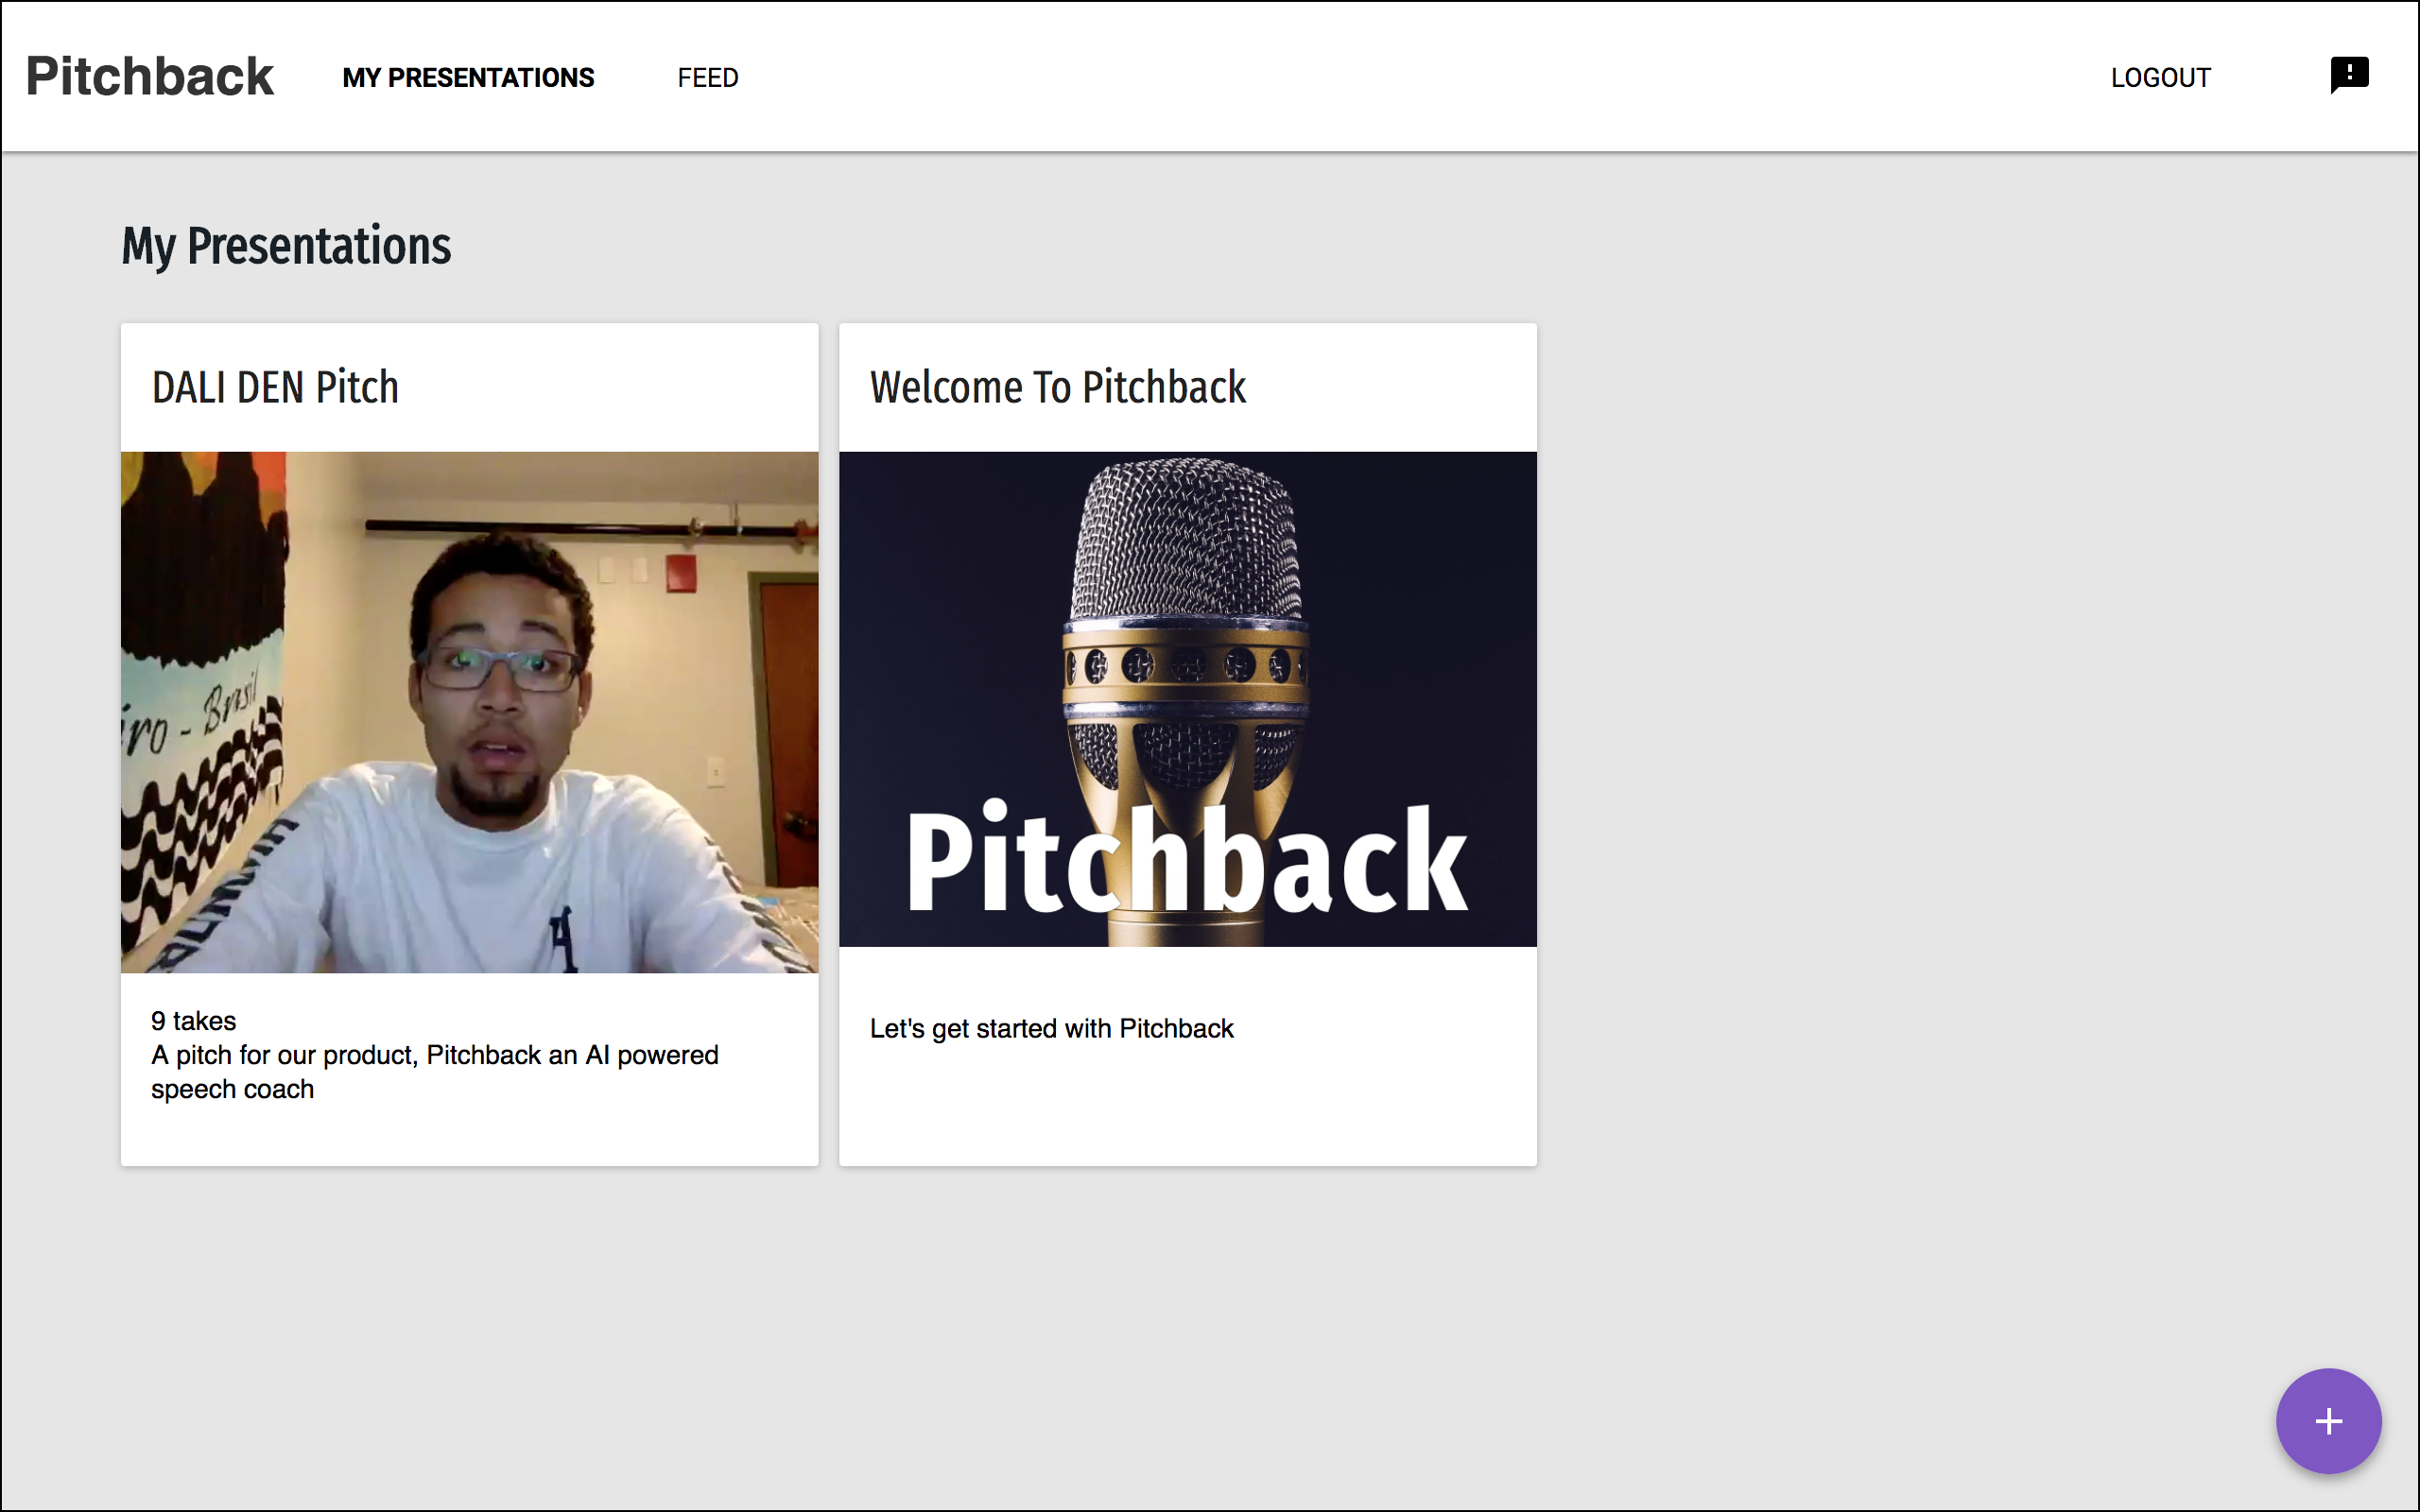
\includegraphics[height=3.7in]{figures/dashboard}
   \caption{The Dashboard View}
\end{figure}

We built a dashboard because we wanted users to create and view multiple
projects. We use a card layout to give a brief overview of the projects that
users have created. Cards imply that there is more information that is not
currently seen. Each of these cards lead to the expanded project view for the
specific project. The preview of the card is the first frame of the last take
the user uploaded for that project to visually remind users of the presentation
content. If there is no video in the project (0 takes) we display the Pitchback
cover photo as shown on the right. In the lower right corner we have a floating
action button indicating that a “create” action is tied to it. The button leads
to the modal view below.

\begin{figure}[H]
  \centering
   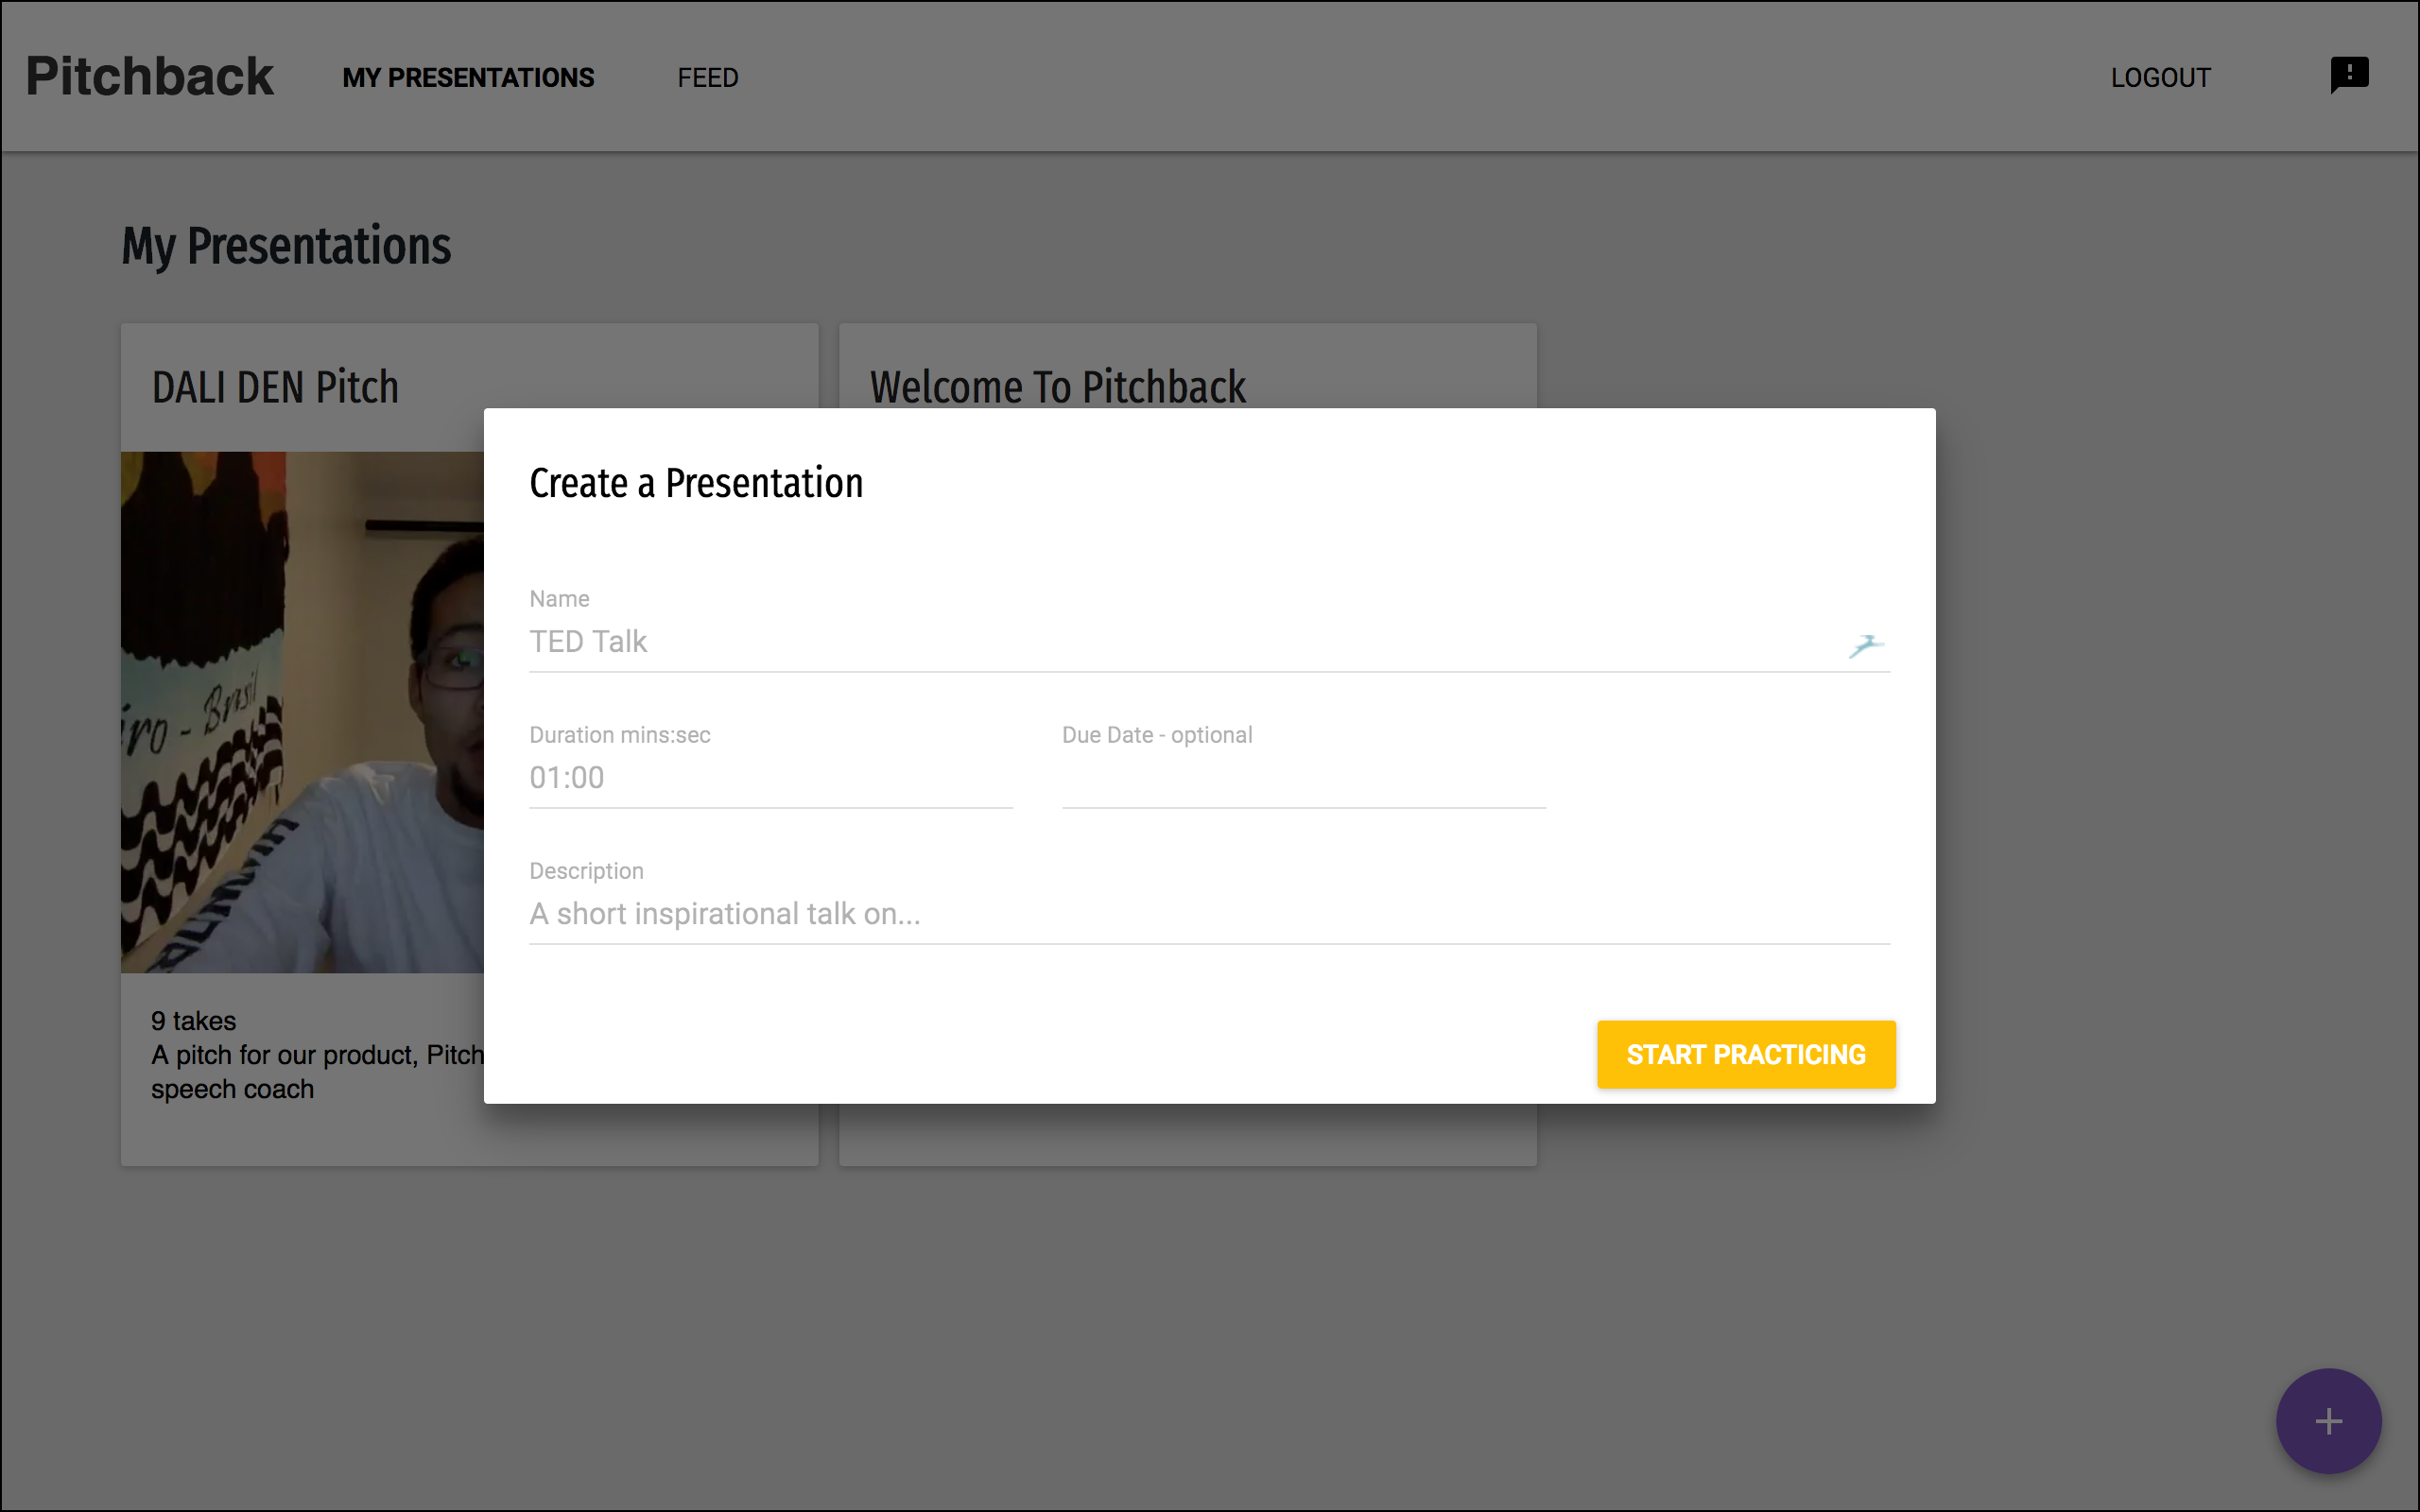
\includegraphics[height=3.7in]{figures/create}
   \caption{Create a Project Modal}
\end{figure}

The dialogue above presents users with a form to provide metadata about their
presentation. The title and description fields are used to display the cards
here on the dashboard and in the later discussed sharing/feed view. 

\subsection*{Project}
\addcontentsline{toc}{subsection}{Project}

\begin{figure}[H]
  \centering
   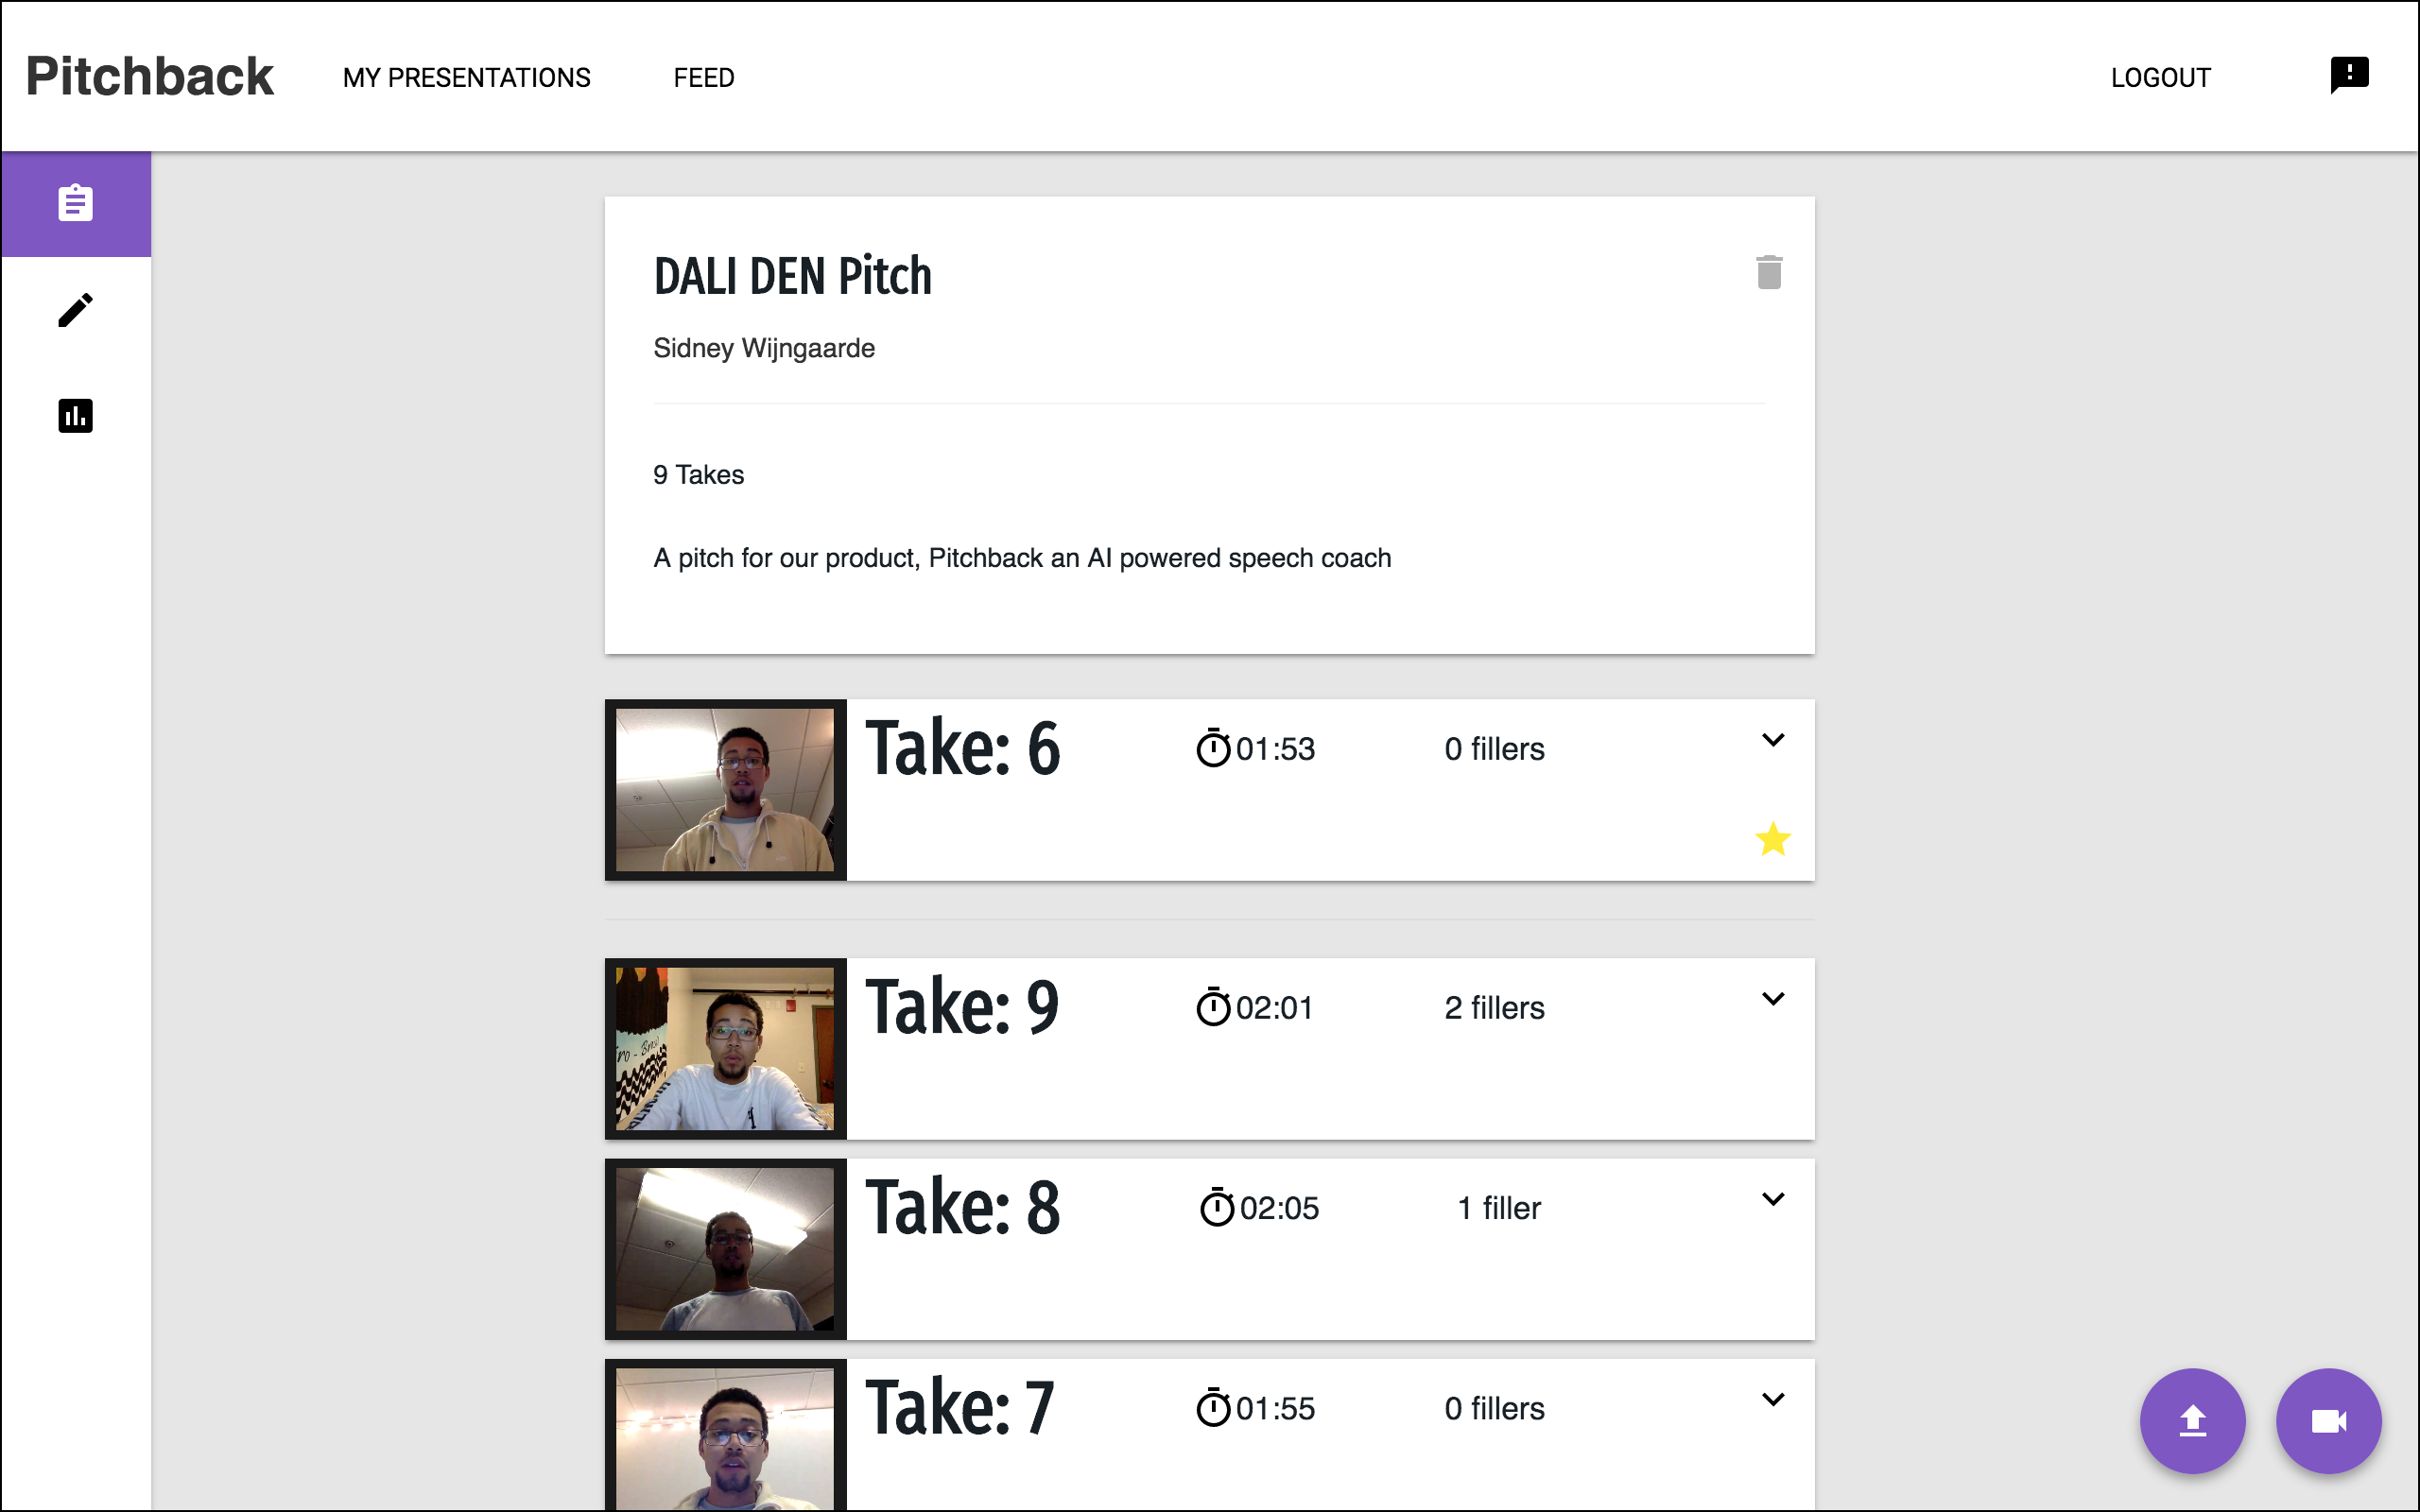
\includegraphics[height=3.7in]{figures/project_collapsed}
   \caption{The Project View}
\end{figure}

We built a project view to allow users to gain access to all of their project
related data in one view. After clicking a card from the dashboard or feed,
users are presented with the project view for that project. This view contains
two subviews. The first (shown above) is the review tab. Here users have
insights into all of the data and insights regarding the current project. At the
top we have the project data card which presents the metadata about the project.
Takes are displayed as cards as well. The takes are organized by date from most
recent to oldest. Users can favorite takes which move them to the top of this
list. The preview image is the first frame of the video to provide a visual
differentiation between the takes. Clicking the take expands the card to reveal
data and comments from other users as shown below.

\begin{figure}[H]
  \centering
   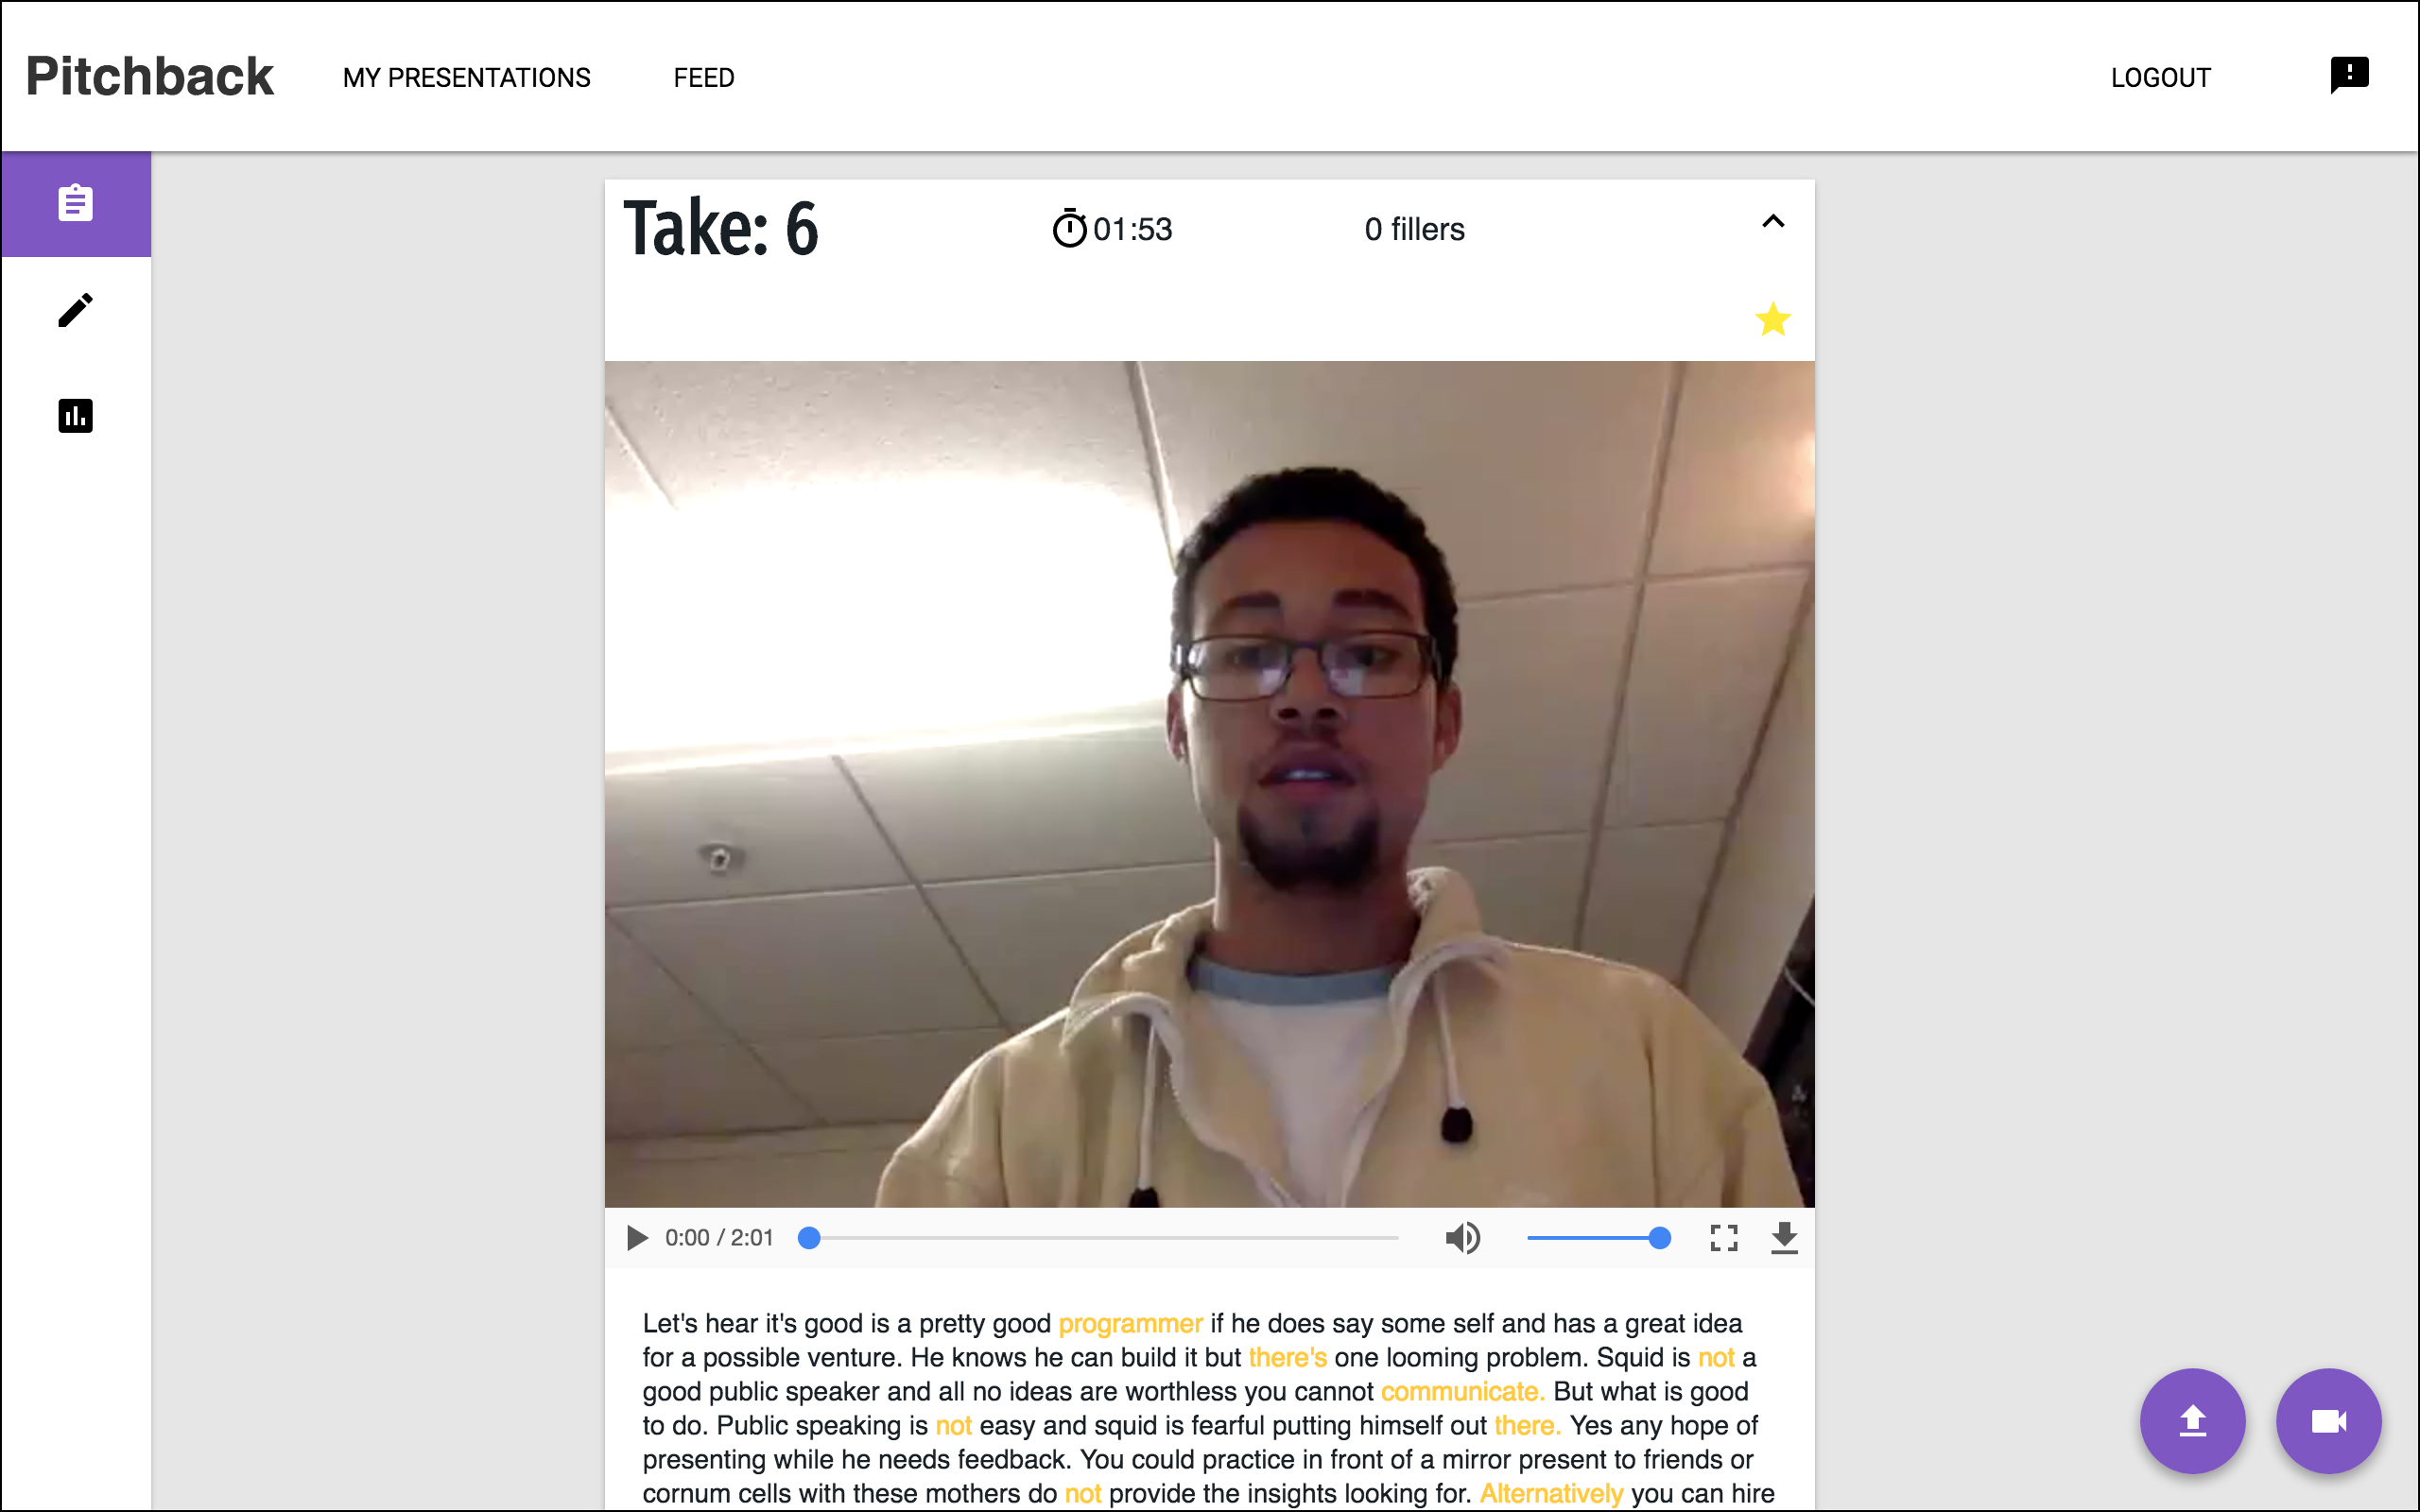
\includegraphics[height=3.7in]{figures/take_1}
   \caption{An expanded take card}
   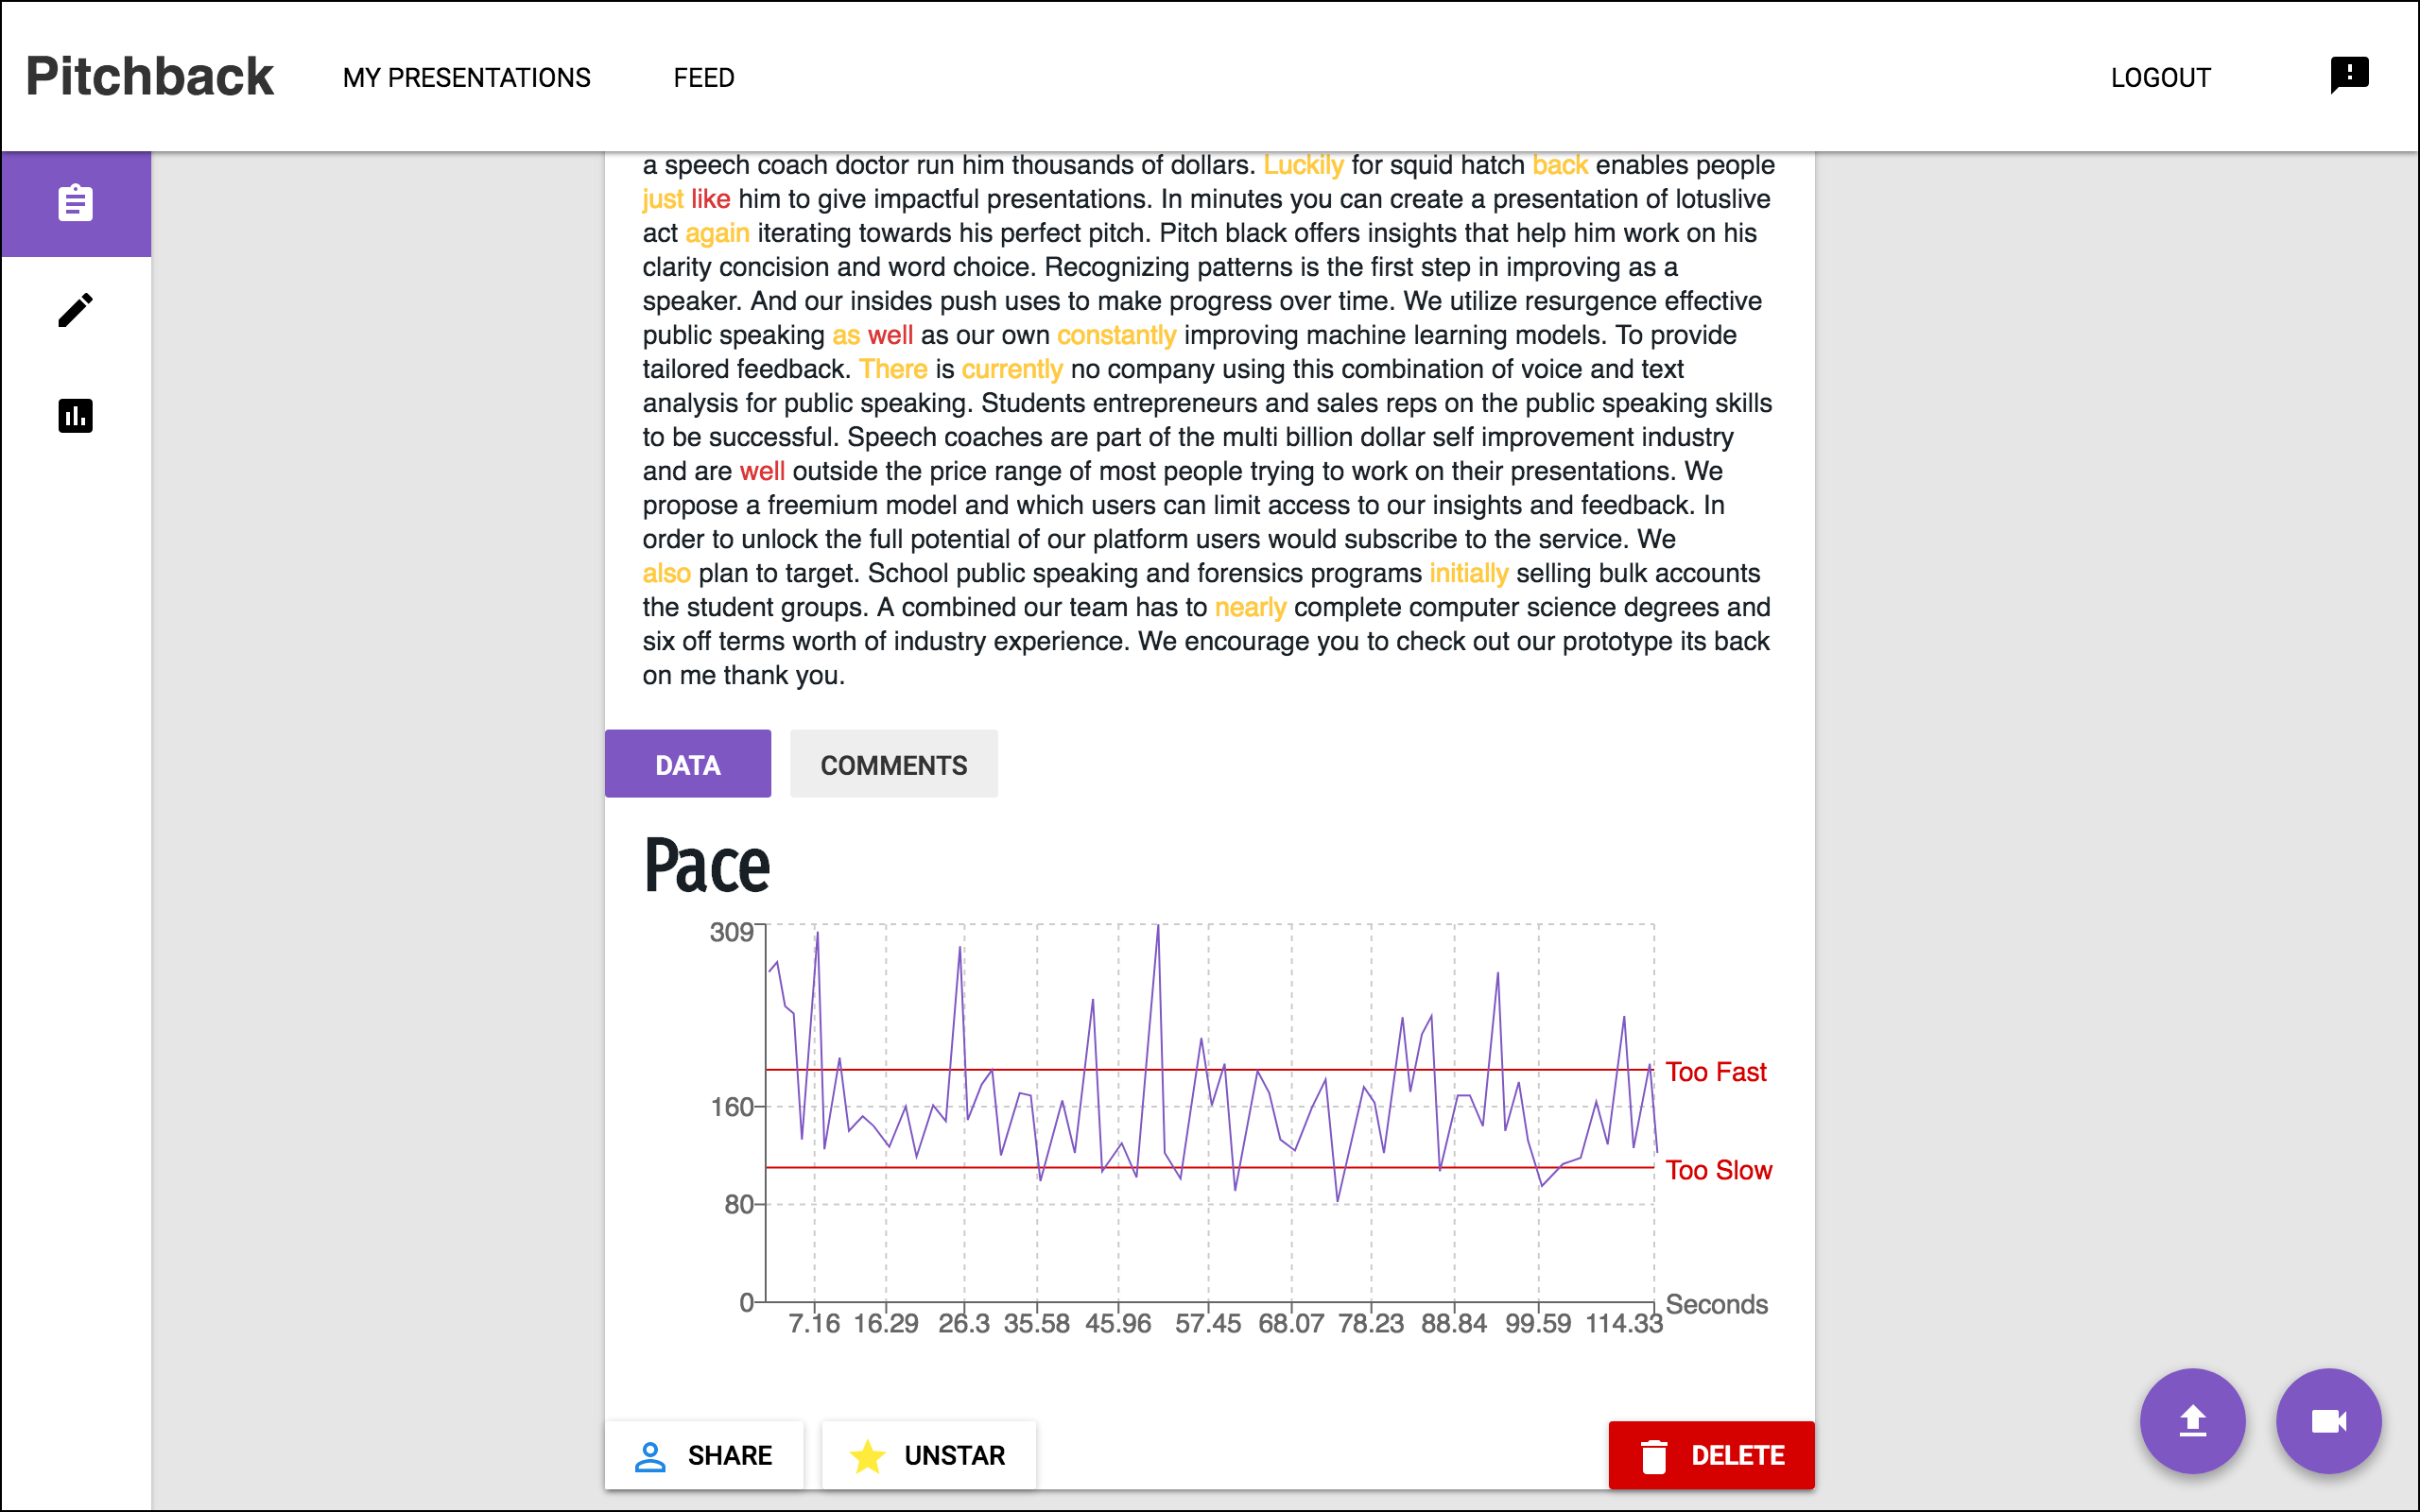
\includegraphics[height=3.7in]{figures/take_2}
   \caption{An expanded take card}
\end{figure}


The users video is followed by a highlighted transcript. The goal of the
transcript is to provide visual cues for Pitchback’s insights as well as provide
a tight feedback loop for users. Users can see the differentiation between
warnings and significant errors at a glance from the color of the highlights.
Hovering over highlighted words reveals a popup with a description of the error
and suggestions for how to improve. Clicking the transcript navigates the video
to where the mistake was made.The users filler words are tallied at the end of
the presentation as well. At the bottom of the card there are two options for
favoriting or sharing the take. Sharing, publishes the take to the general feed
and gives other users on the platform access to the full take card. These other
users can leave comments as well.

There are two floating action buttons at the bottom right of the view. The first
launches an upload dialogue. Users can drag and drop in a previously recorded
video to be analyzed by pitchback. This is useful for analyzing real
presentations from the web or given and recorded by the user elsewhere. The
second action button launches the in-site recording view.

\subsection*{Record}
\addcontentsline{toc}{subsection}{Record}

\begin{figure}[H]
  \centering
   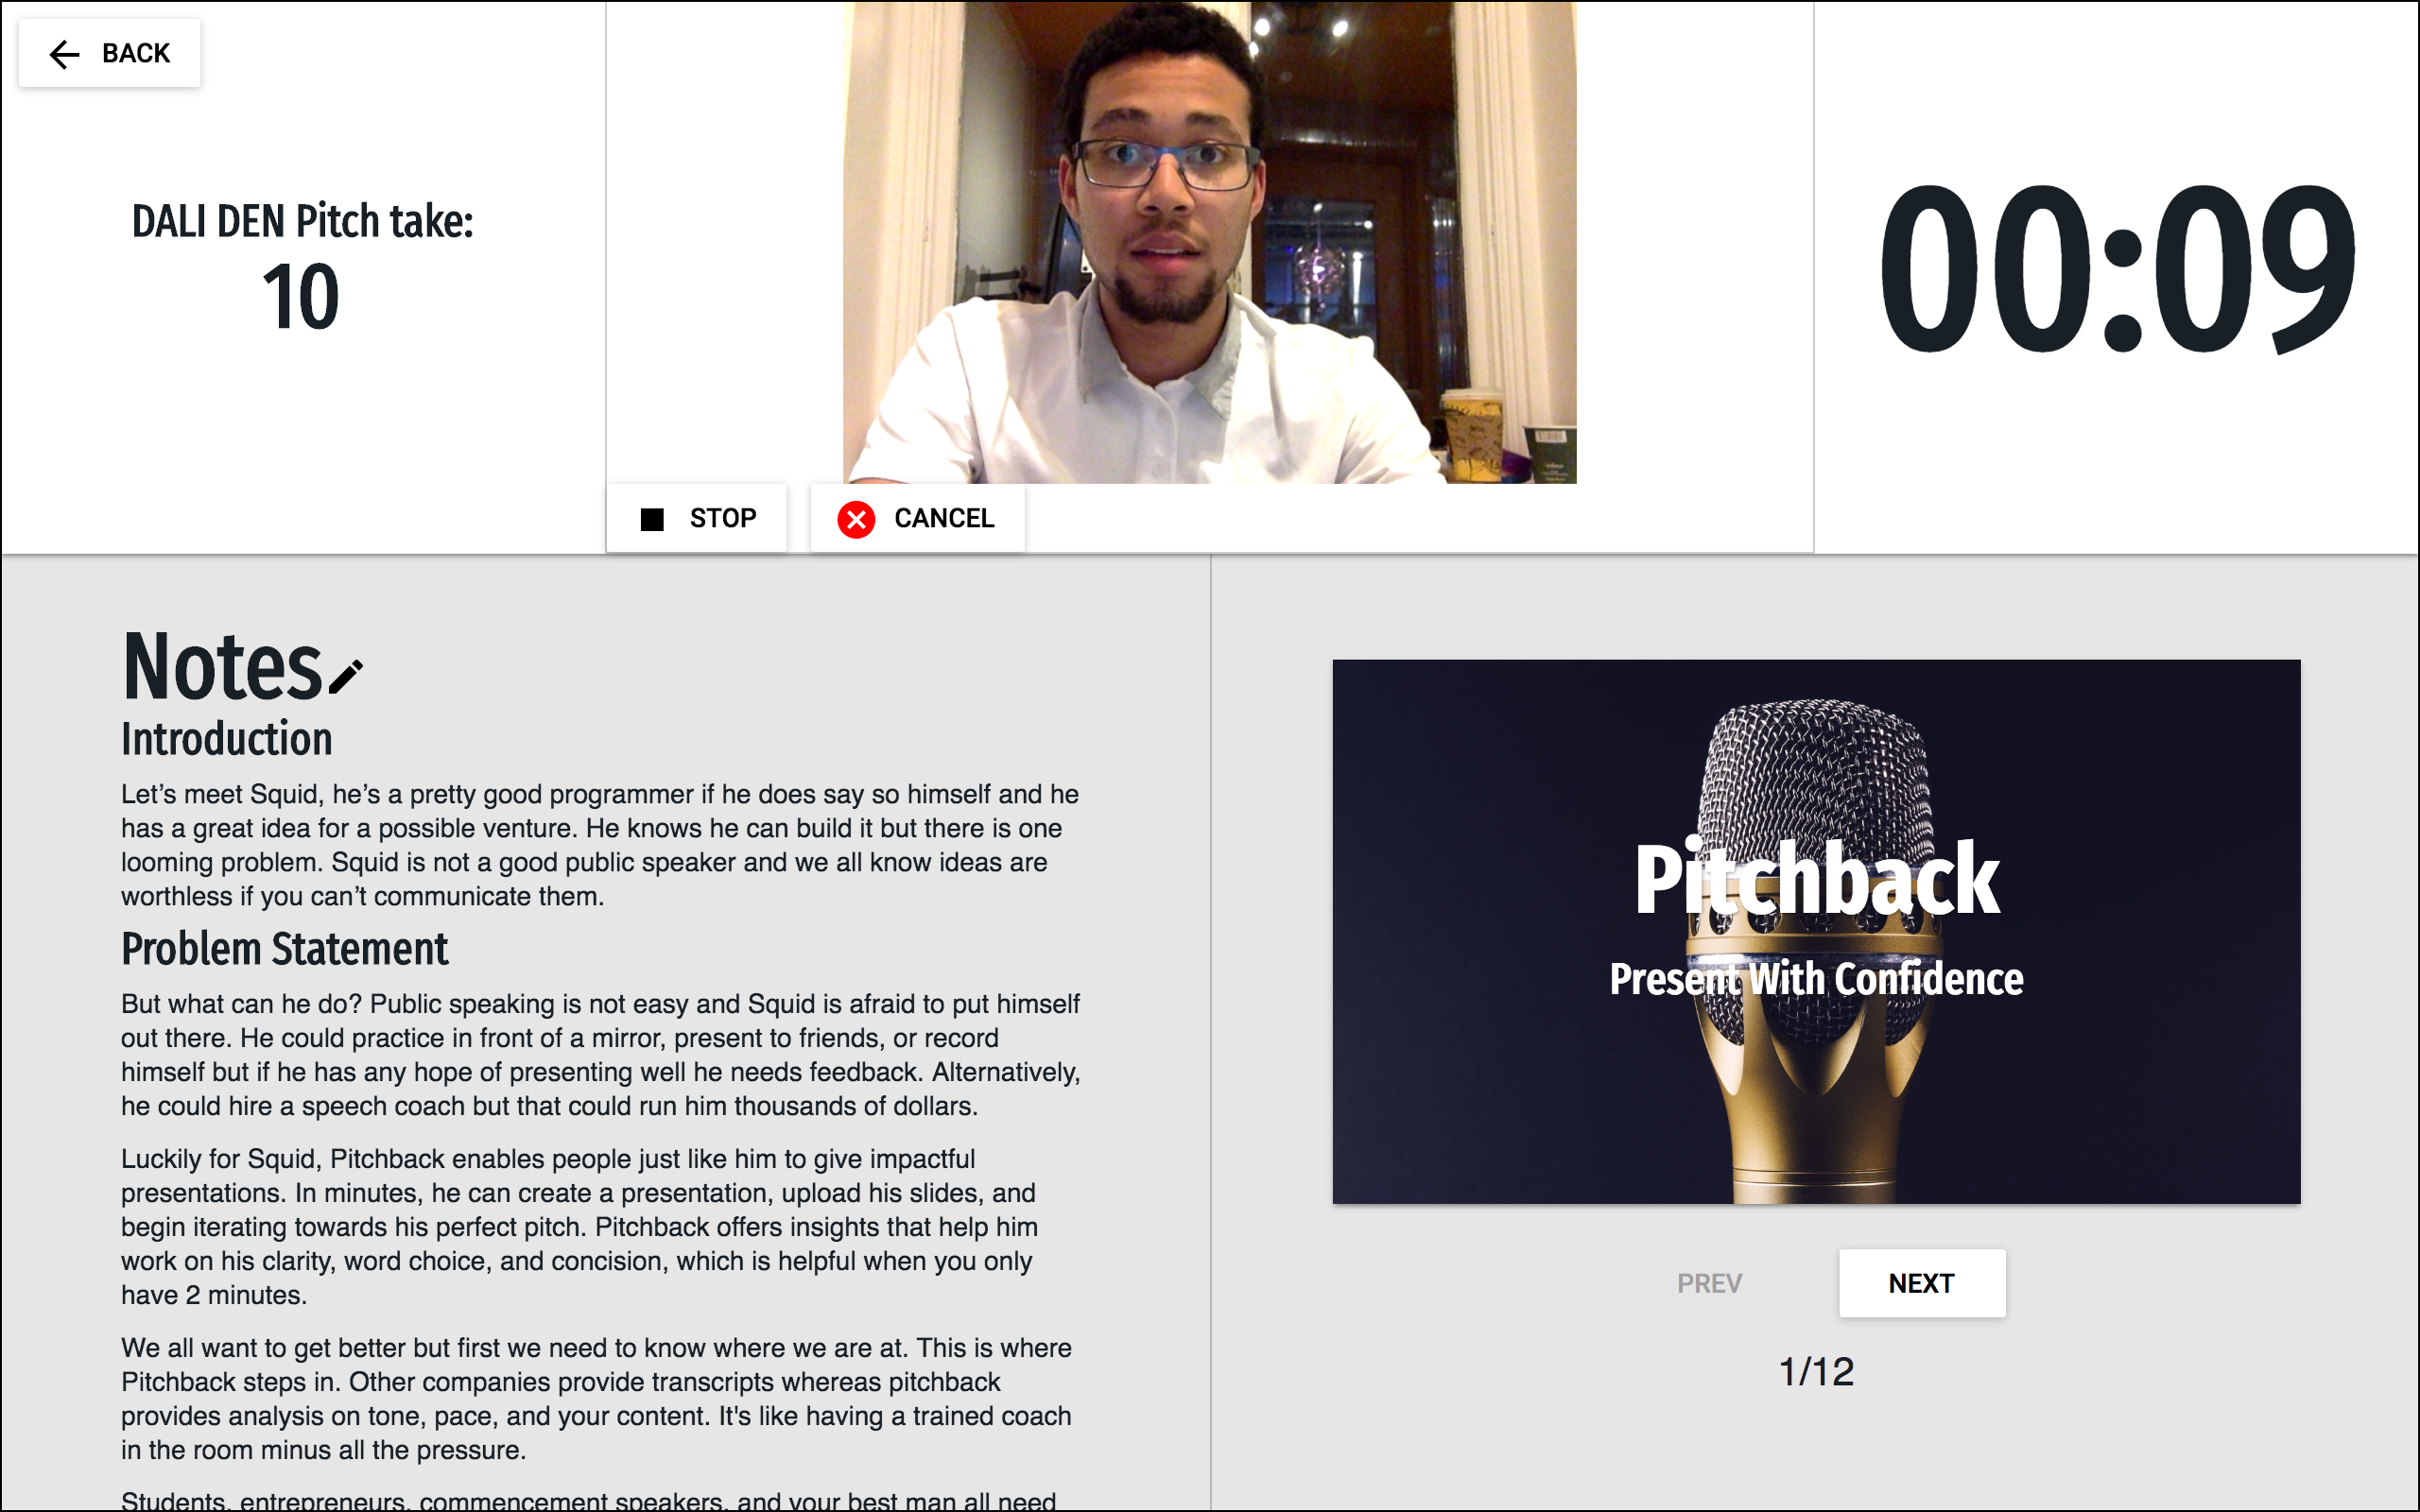
\includegraphics[height=3.7in]{figures/record}
   \caption{The Record View}
\end{figure}

Recording in-site gives users access to their presentation materials during a
practice session. Users can watch themselves record while keeping an eye on the
time, their slides, and notes. The view allows users to practice clicking
through their slideshow. Users can review the take before they choose to upload
it to the platform.

Once users upload a take they are pushed back to the review tab of the project
view. The takes transcript begins to fill in as the video is being processed in
order to make the ui feel faster and more responsive. This method of displaying
intermediate results greatly increased the usability of the platform.

\begin{figure}[H]
  \centering
   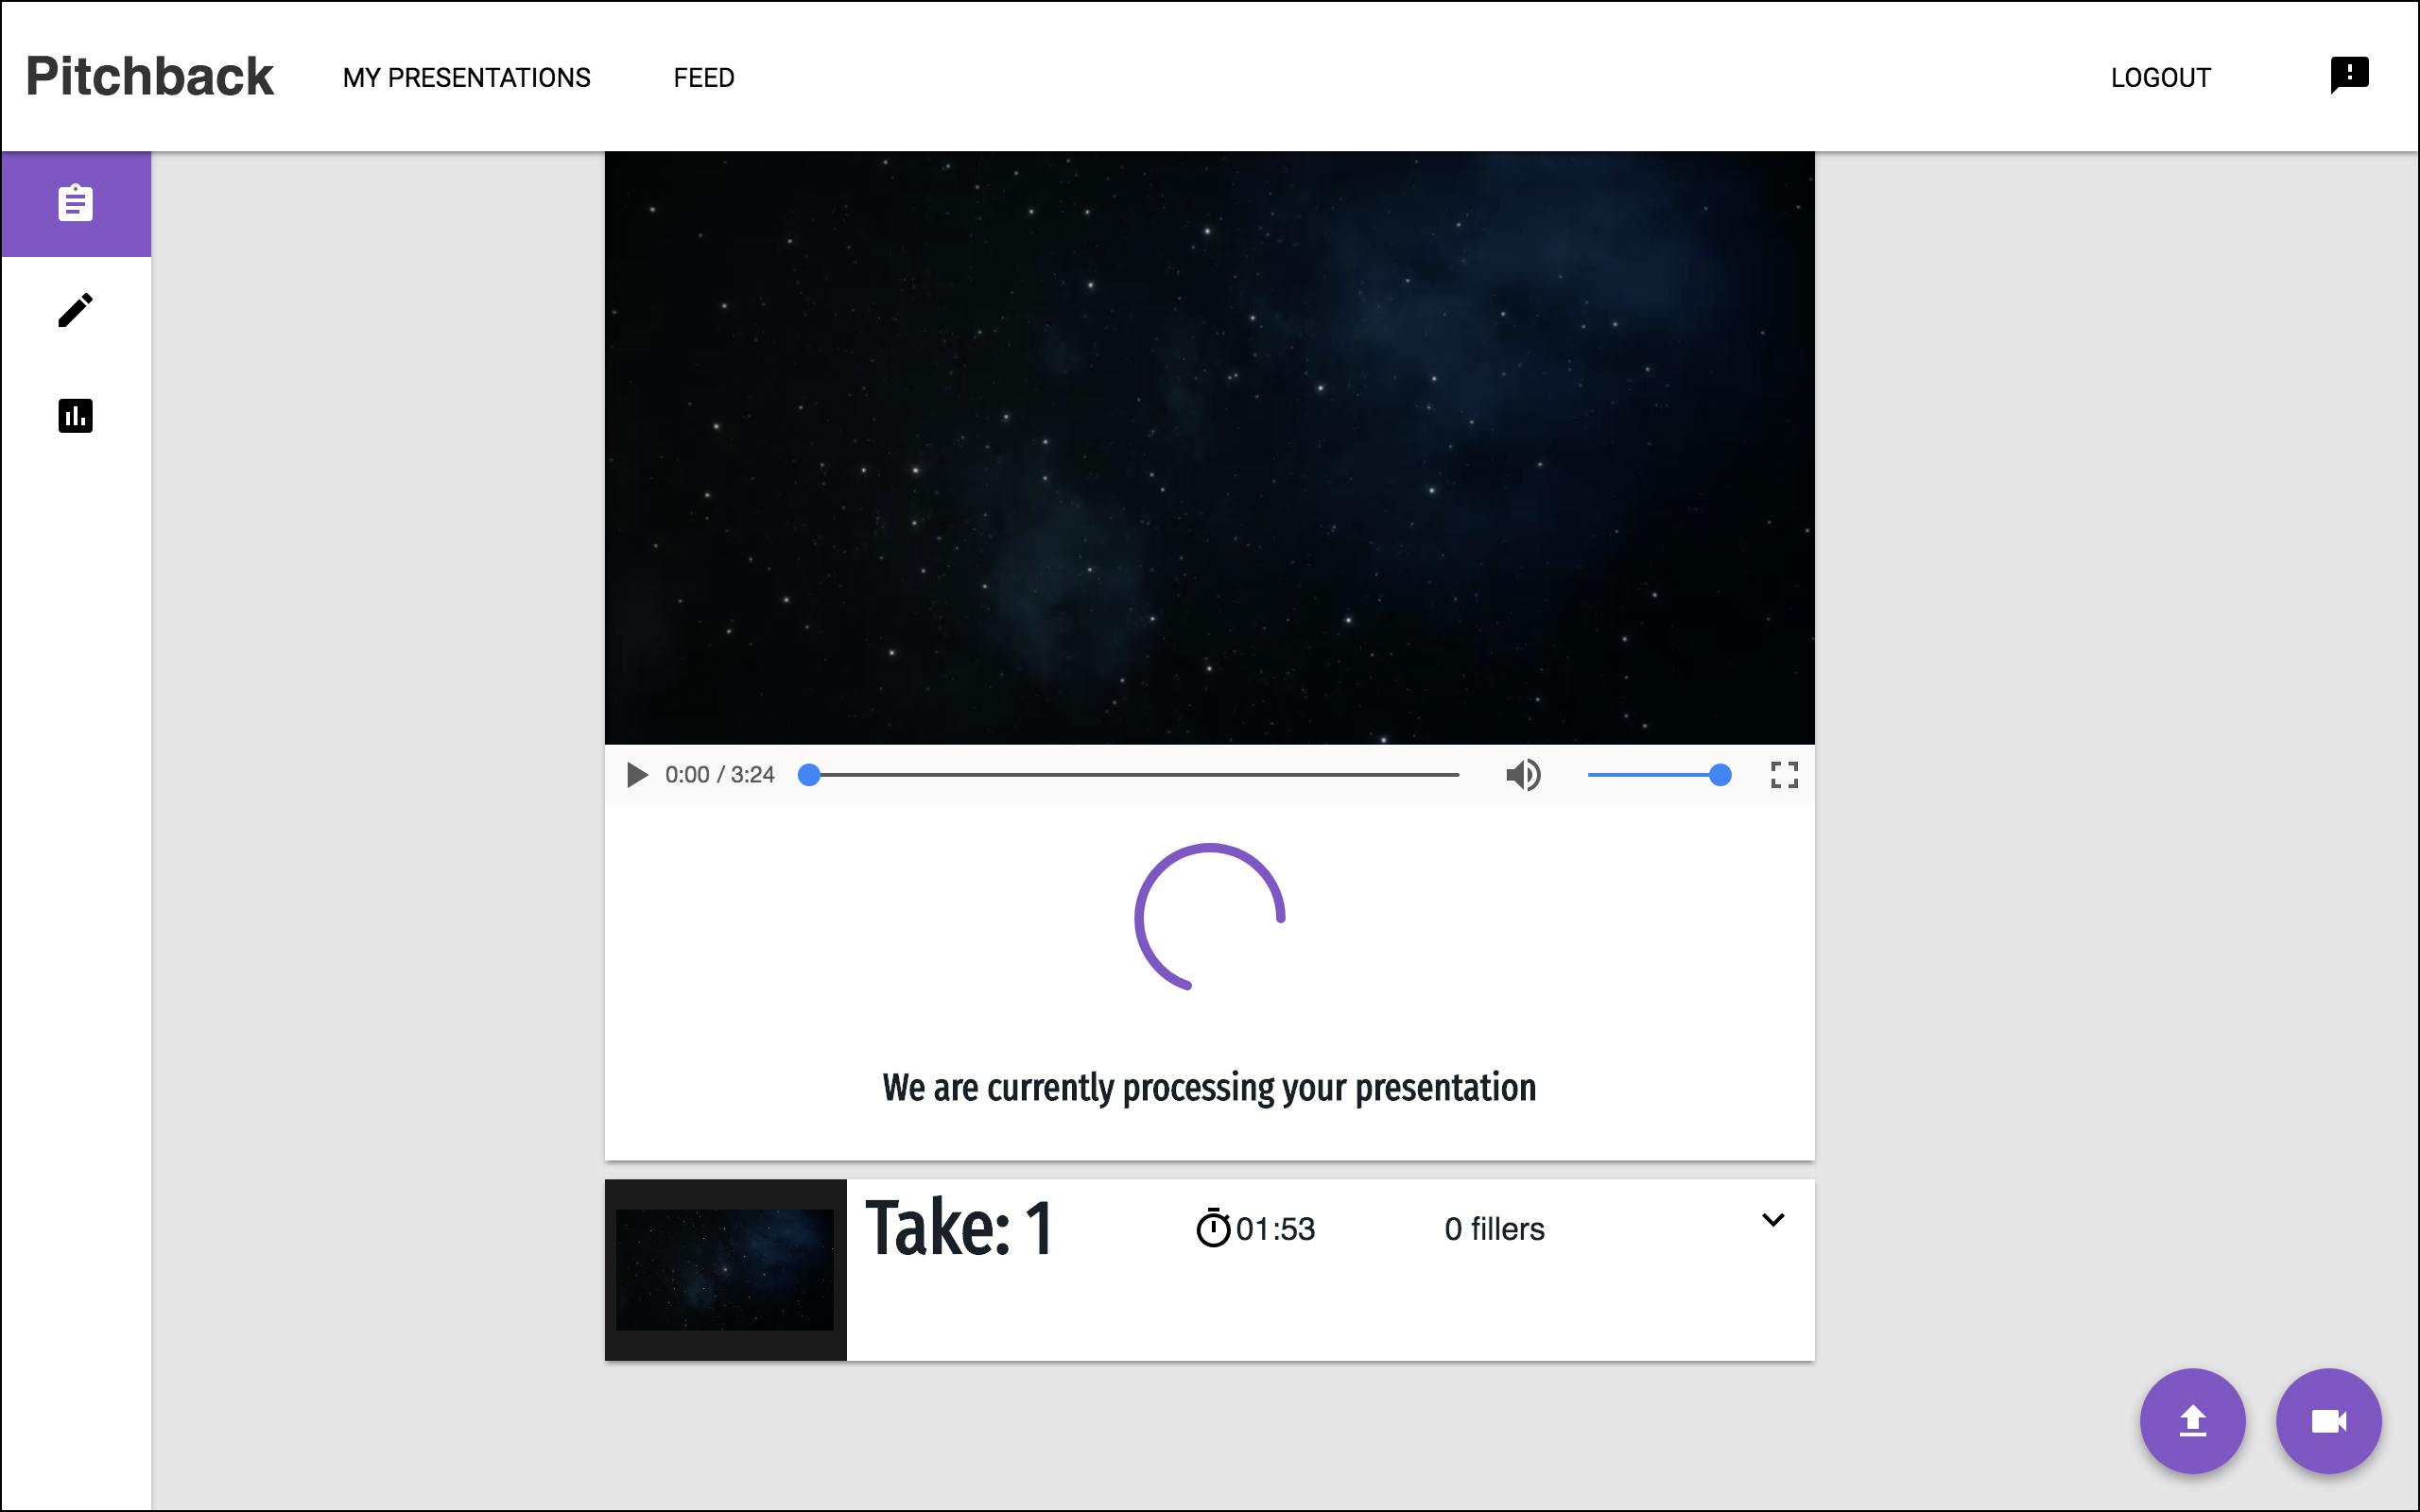
\includegraphics[height=2.7in]{figures/processing_1}
   \caption{Initial Loader Before Intermediate Results are Received}
   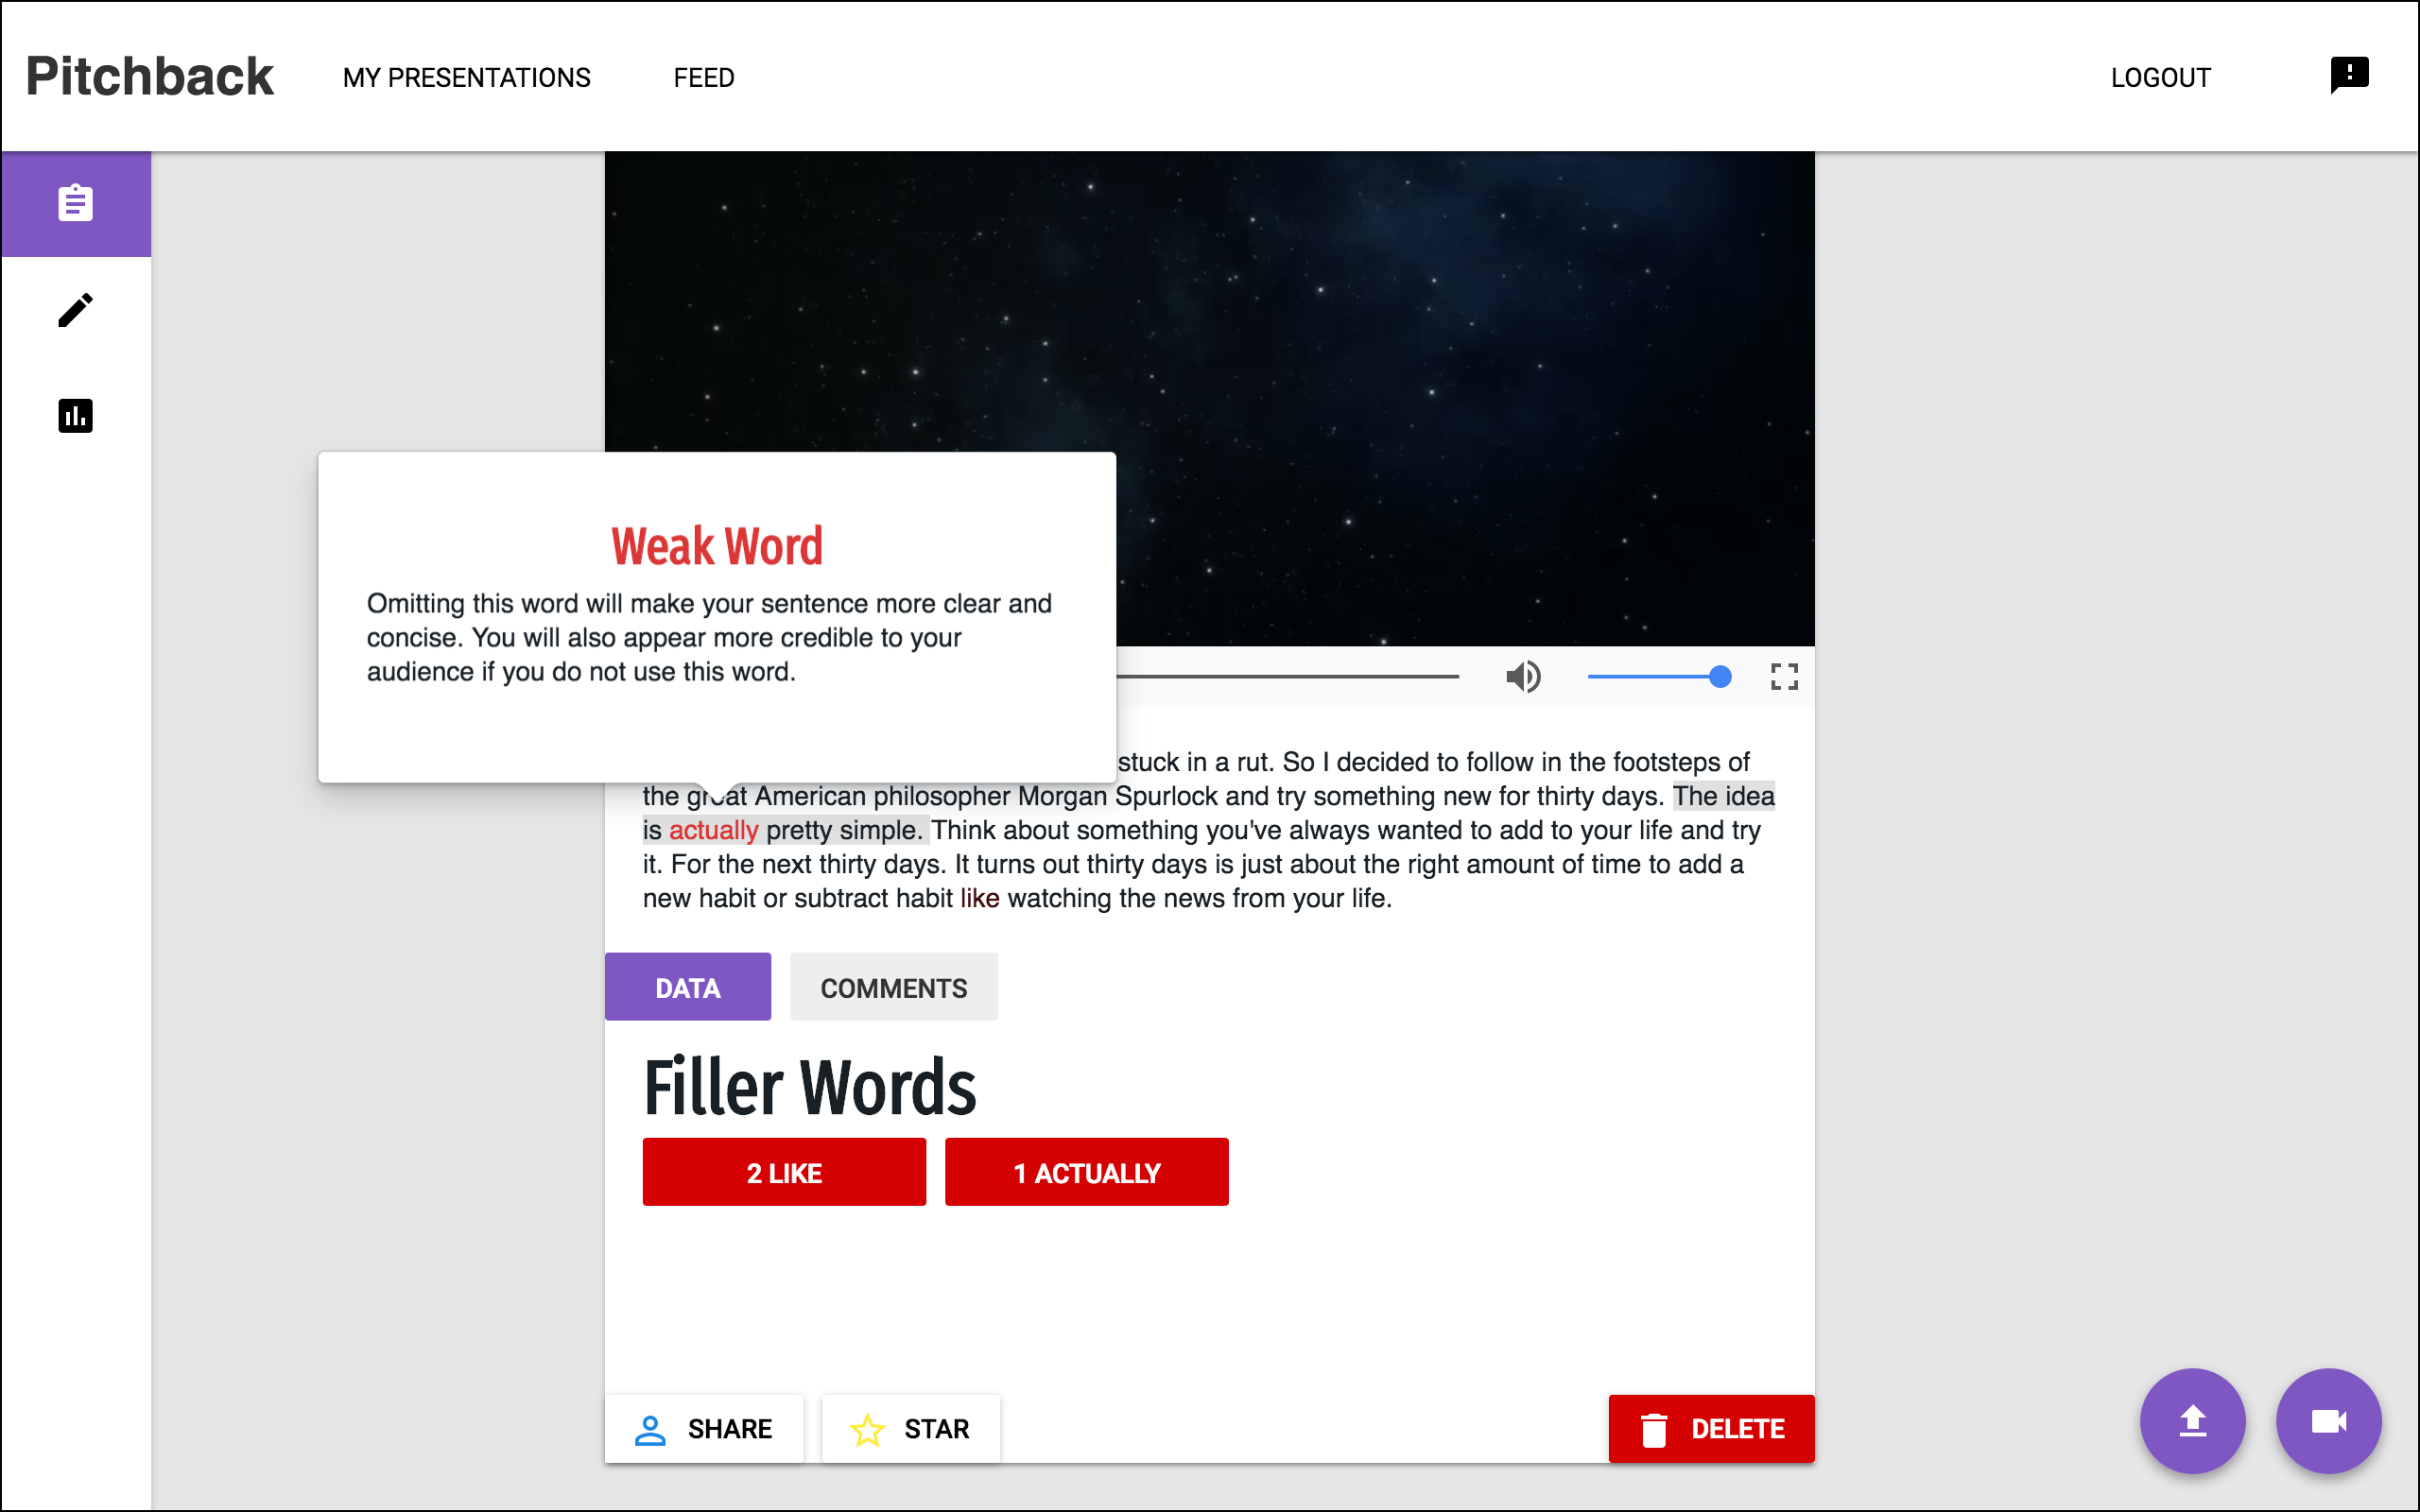
\includegraphics[height=2.7in]{figures/processing_3}
   \caption{A Partially Populated Transcript with Insights}
   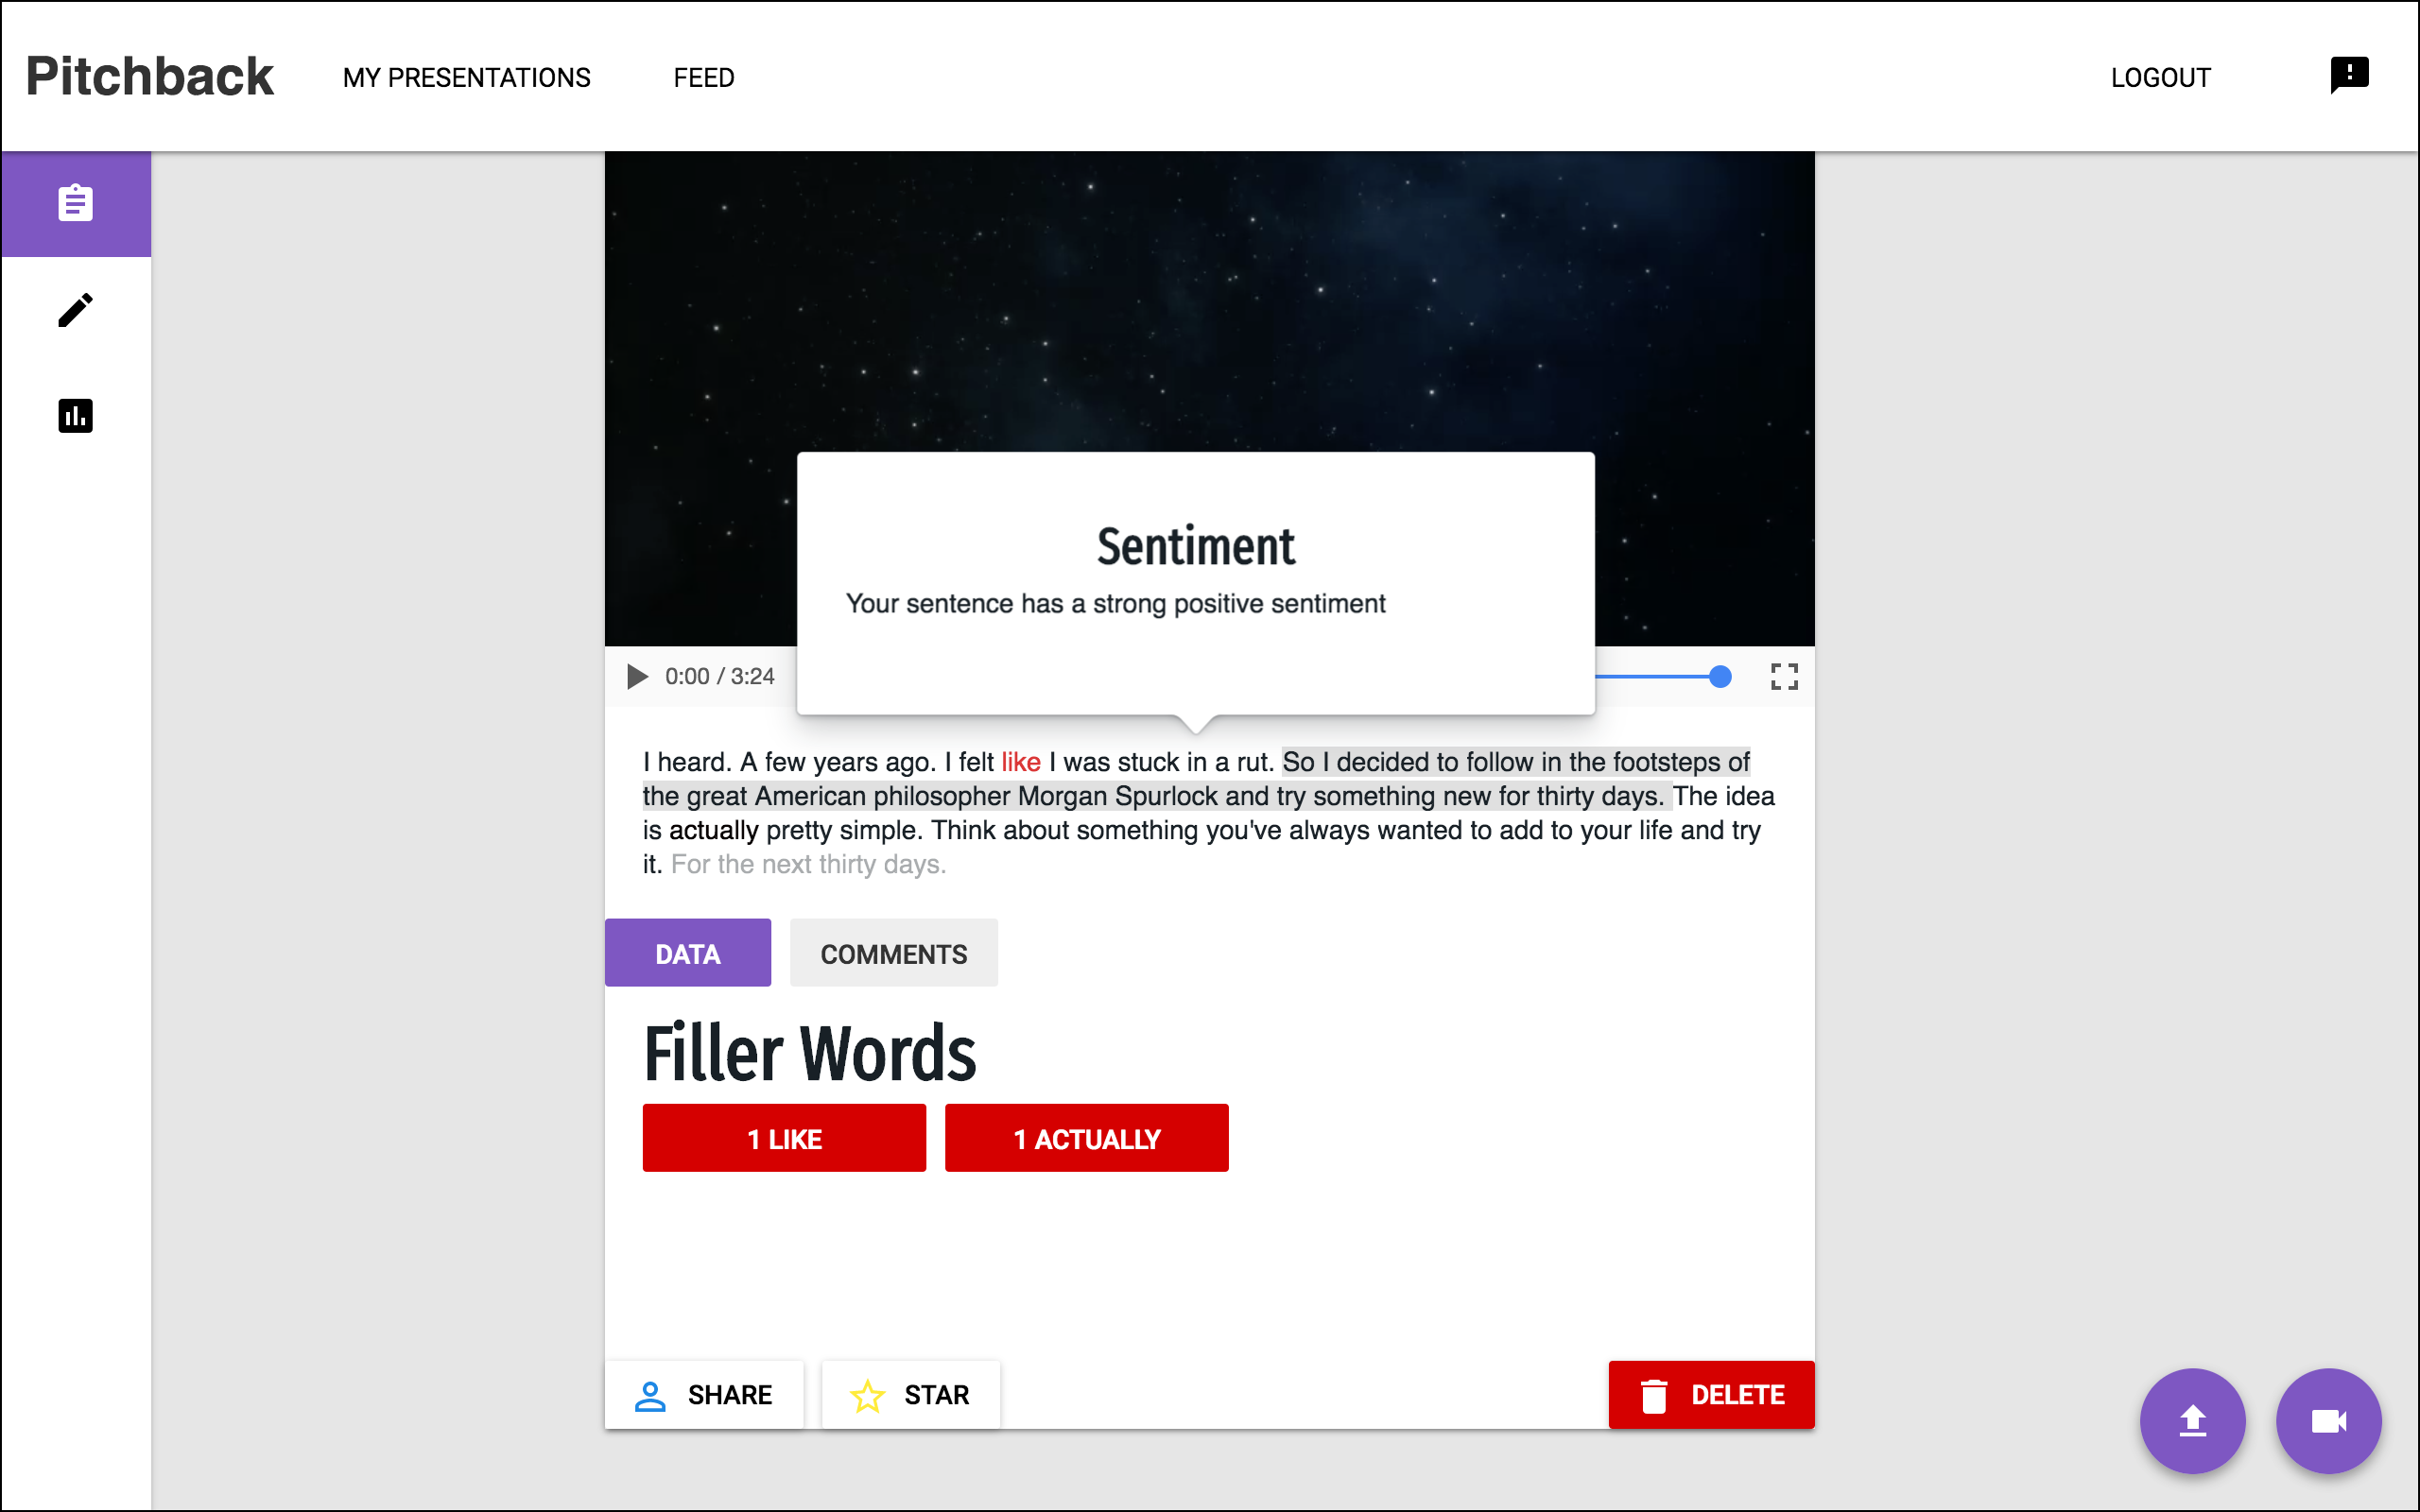
\includegraphics[height=2.7in]{figures/processing_2}
   \caption{A Partially Populated Transcript}
\end{figure}

\subsection*{Feed}
\addcontentsline{toc}{subsection}{Feed}

\begin{figure}[H]
  \centering
   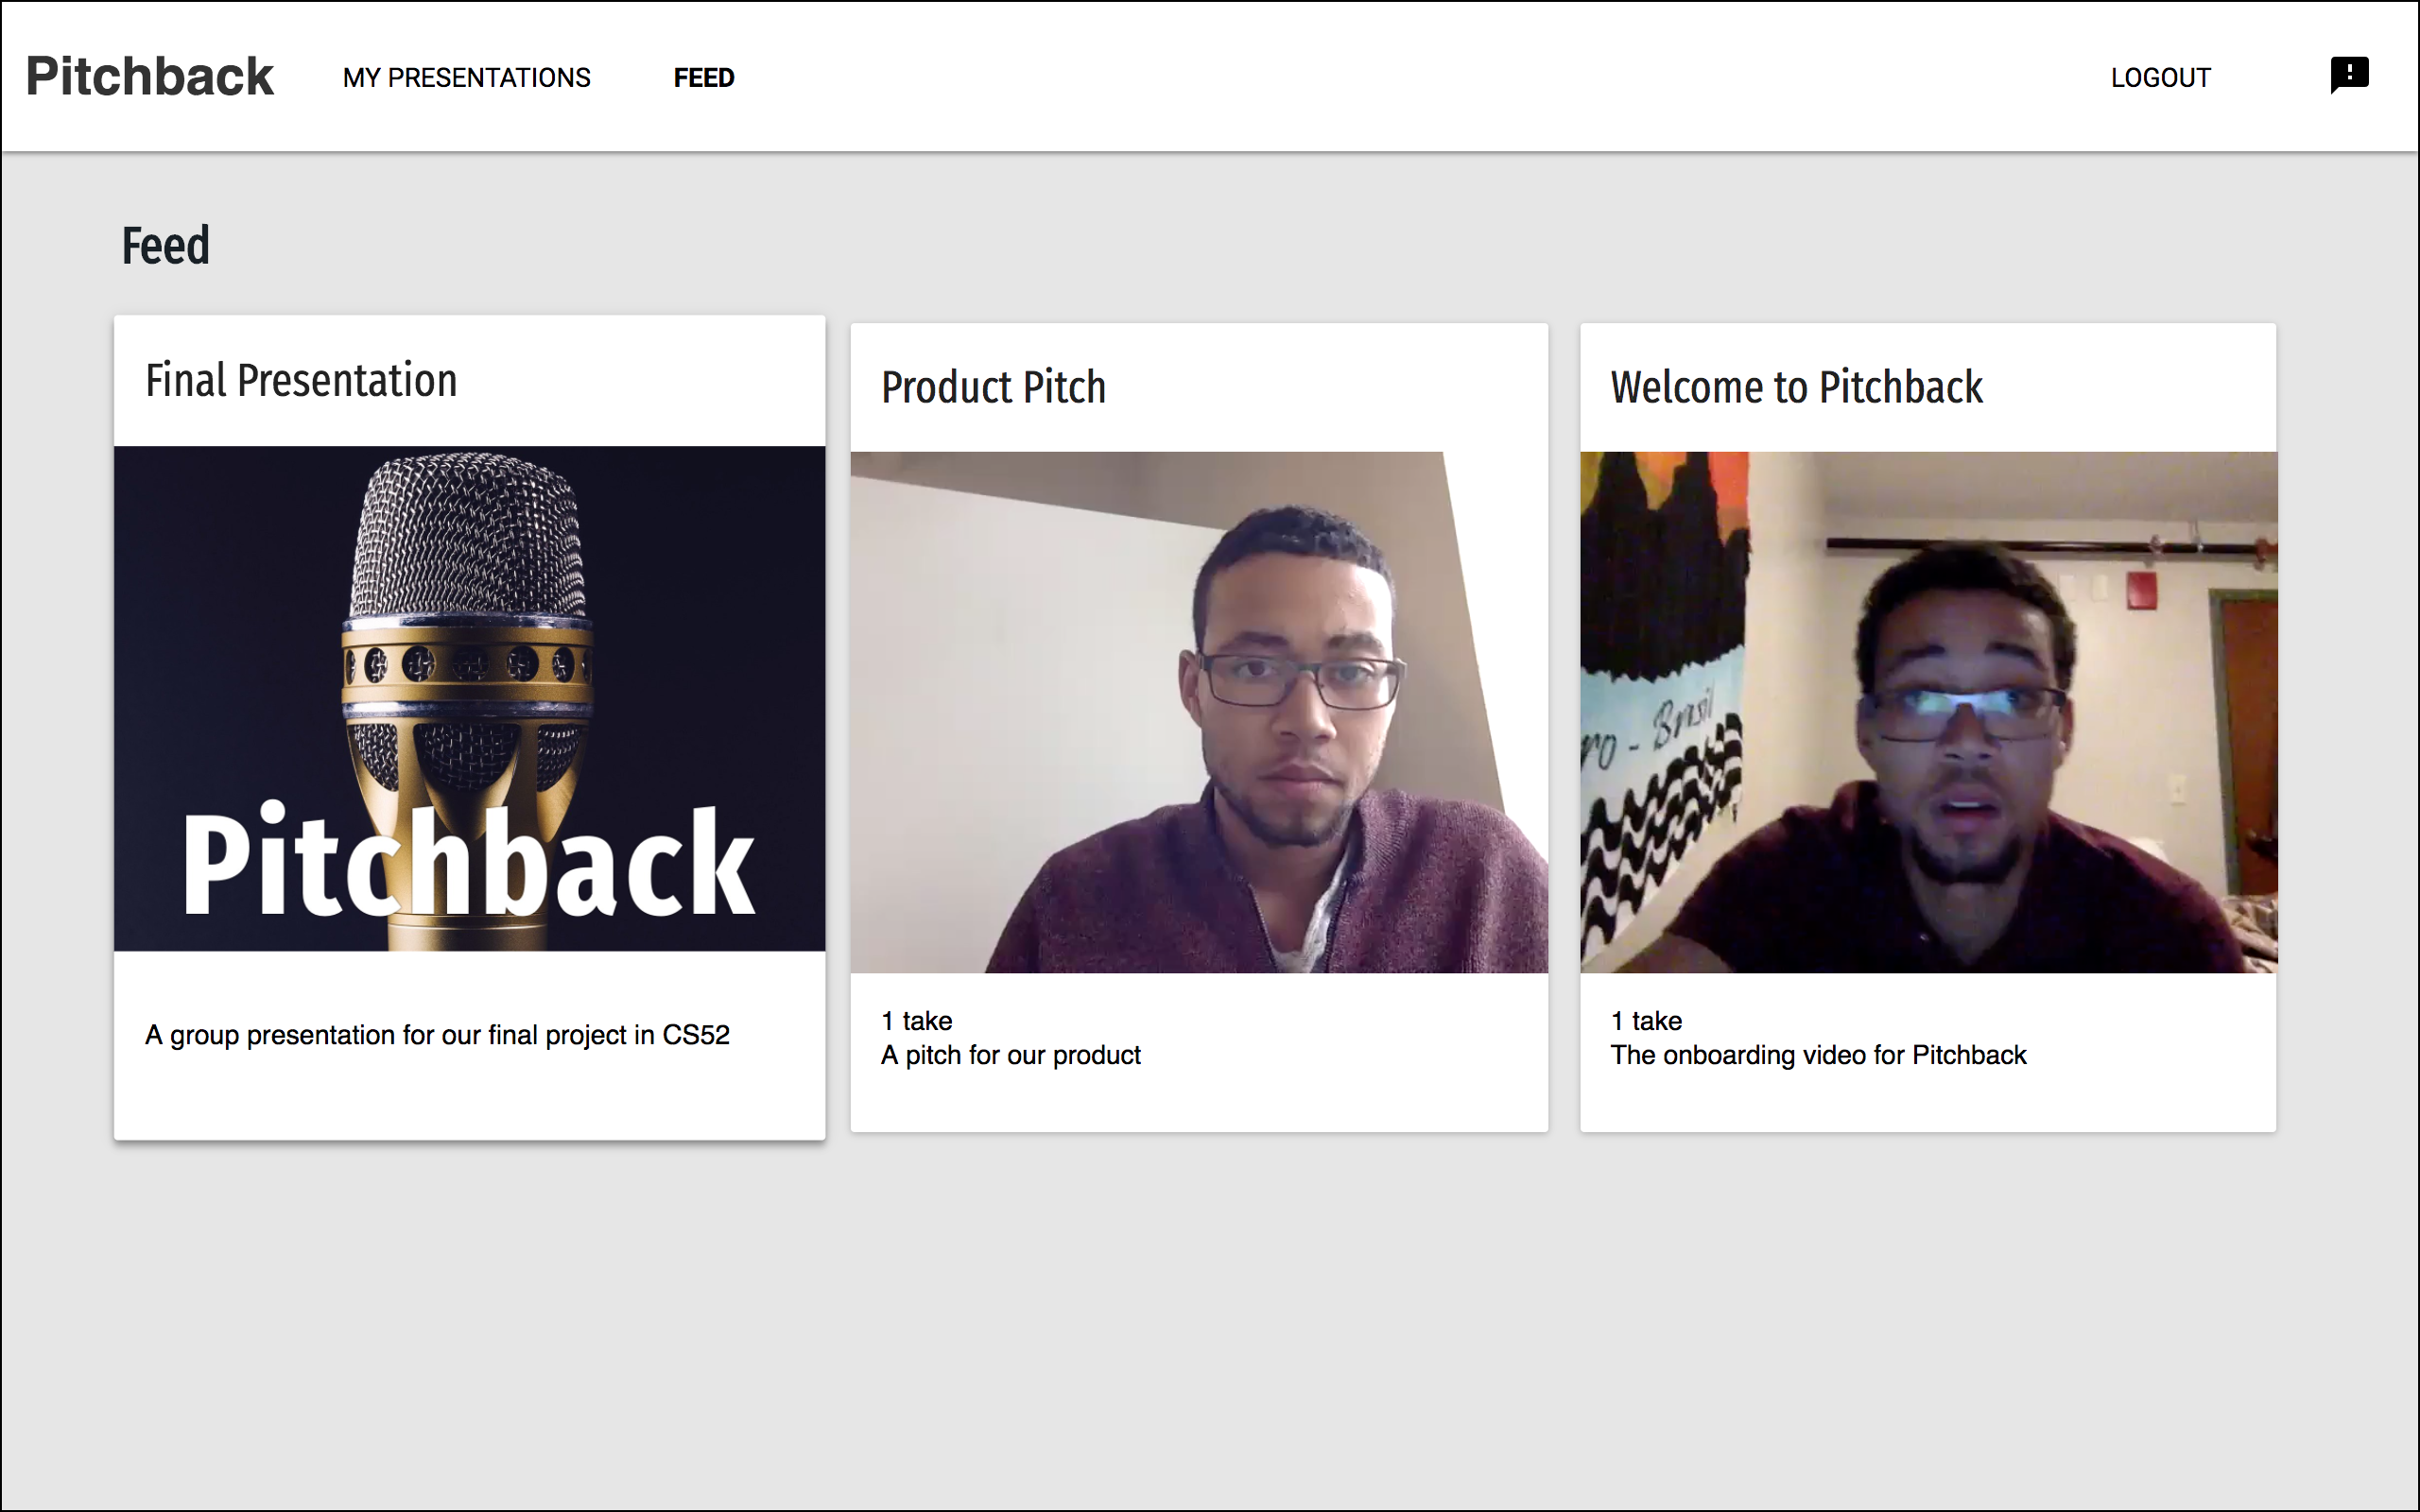
\includegraphics[height=3.7in]{figures/feed}
   \caption{The Feed View}
\end{figure}

The \textit{Feed} view facilitates the peer review process by collecting public
presentations. Presentations that show up in the feed view have at least one
take that has been published for review. This view allows users to discover new
content on the platform.

\section*{IMPLEMENTATION} \label{chapterimplementation}
\addcontentsline{toc}{section}{Implementation}

% Talk about your technical implementation here. Assume a general CS audience that doesn't require explanation of datastructures or basic algorithms, but does not know your specific area.
In building Pitchback as a modern web platform we considered many design
patterns for the architecture of our data processing system. This chapter
highlights tradeoffs and design choices as well as the technologies in use.

\subsection*{Data Structures}
\addcontentsline{toc}{subsection}{Data Structures}

To support the processing and display of presentation data we implemented three
key data structures: project, revision, and transcript. The transcript tree
contains nodes in a hierarchical order of types: transcript, sentence, and word.

\begin{figure}[H]
  \centering
   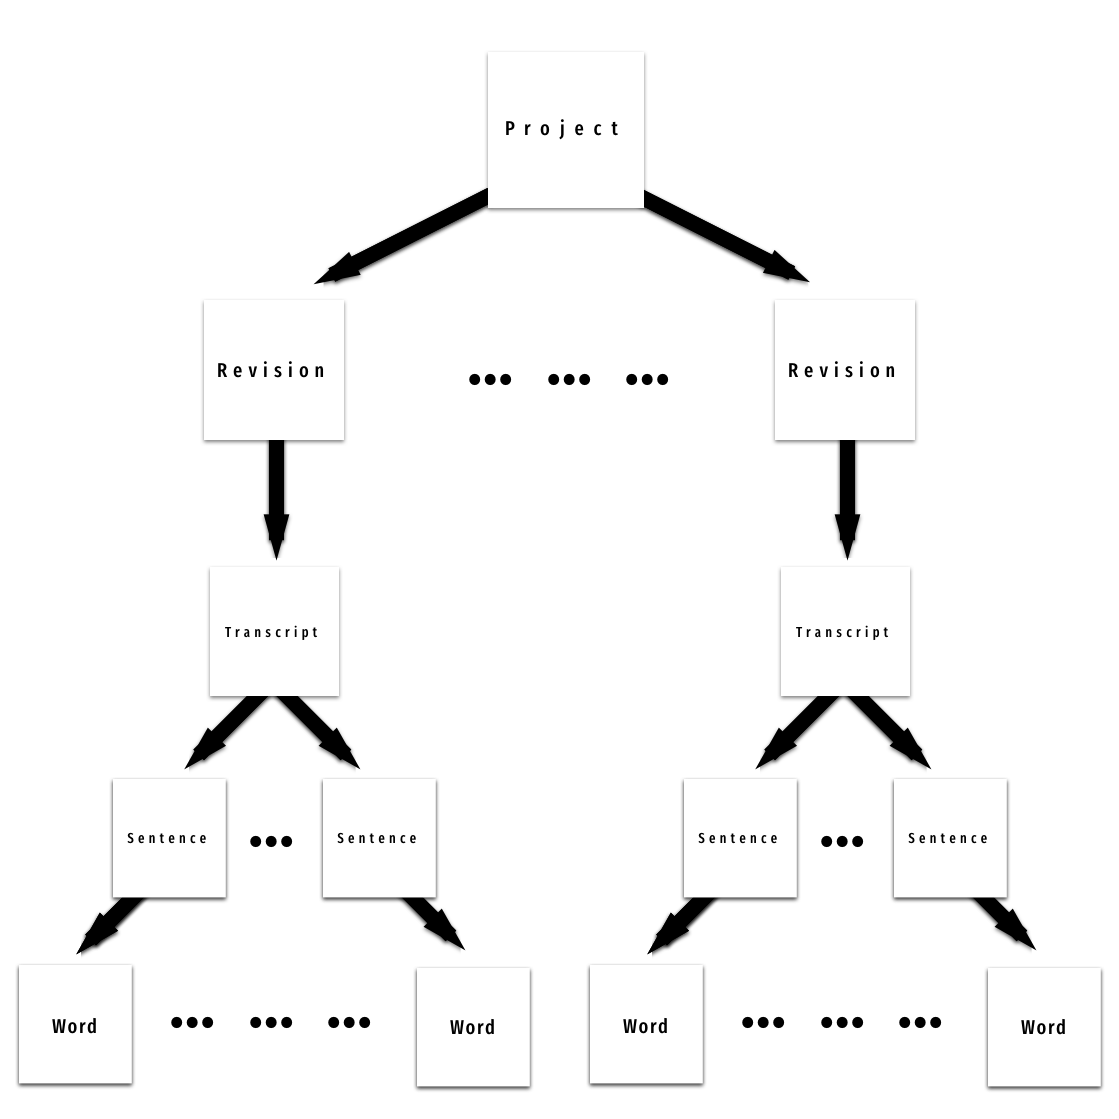
\includegraphics[height=6.3in]{figures/datastructures}
   \caption{Data Structures}
\end{figure}

\subsubsection*{Project}
\addcontentsline{toc}{subsubsection}{Project}

The project data structure is the top level node of a multiple revision tree.
The project schema holds references to each revision in the project as well as
project metadata. Finally the project node stores markdown notes as well as a
link to the users slides stored on S3. The schema is as follows:

\textbf{name} String respresenting the title of the project.

\textbf{description} String providing a description of the project.

\textbf{duration} Integer target time for the presentation.

\textbf{slides} String URL for user slides stored on \textbf{Amazon S3}

\textbf{revisions} Array of revisions (see schema below)

\subsubsection*{Revision}
\addcontentsline{toc}{subsubsection}{Revision}

The revision data structure is the next node in the project tree hierarchy. The
data for each take uploaded by the user is stored in the revision database
structure. In each revision metadata such as whether or not it is starred or
published is stored. This structure also stores the transcript tree - the core
data structure behind Pitchbacks presentation insights. Finally, the processing
field is used to signal the client as to whether or not there is more data to
render. The schema is as follows: \textbf{name} String respresenting the title
of the project.

\textbf{published} Boolean indicating if the revision is public

\textbf{starred}: Boolean indicating if the revision is favorited

% \textbf{processing}: { status:  one of processing, error, finished },
\textbf{words}: Array of Strings containing the words transcribed for this revision

\textbf{transcript}: Transcript schema discussed below,

\textbf{videoURL}: String URL for the video stored on \textbf{Amazon S3}

\textbf{comments}: Array of comments

\subsubsection*{Transcript}
\addcontentsline{toc}{subsubsection}{Transcript}

\begin{figure}[H]
  \centering
   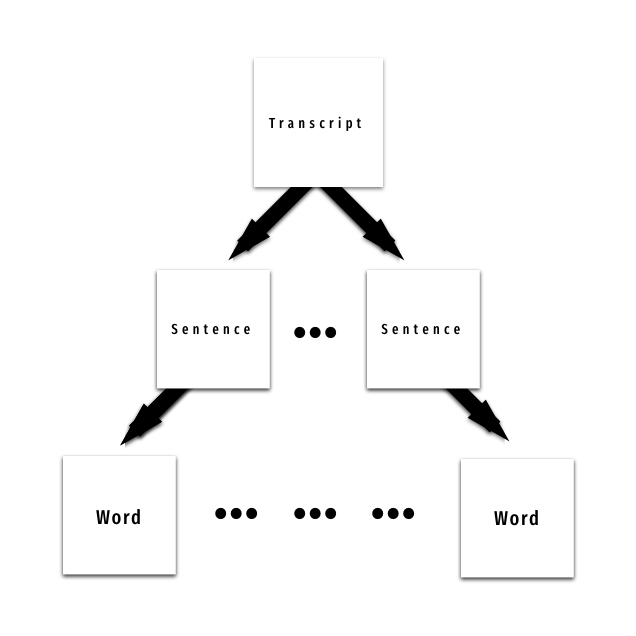
\includegraphics[height=6.3in]{figures/transcript}
   \caption{Data Structures}
\end{figure}

We implemented the transcript rooted tree data structure to allow for the
processing and storage of presentation transcripts in a way that preserves its
hierarchical nature. There are currently three types of nodes in this tree
structure: transcript, sentence, and, word. The root node is the only transcript
node in the tree. This node maintains an ordered list of sentence nodes as
children. Similarly, sentence nodes contain an ordered list of word nodes as
children. Finally, word nodes are leaf nodes in the tree. Each node in the tree
contains the same data fields. The schema is as follows:

\textbf{key} String unique id for the node,

\textbf{type}: String one of transcript, sentence, or word,

\textbf{index}: Array of two elements: start index and end index

\textbf{children}: Array of child transcript nodes,

\textbf{features}: Hash Table of features to counts

\textbf{timestamps}: Array of two elements: start time and end time

The transcript class is implemented as a functor, or simply a class that
implements map. The map function accepts a function as an argument and applies
the function to each node of the tree during a depth first traversal.

\begin{figure}[H]
  \centering
   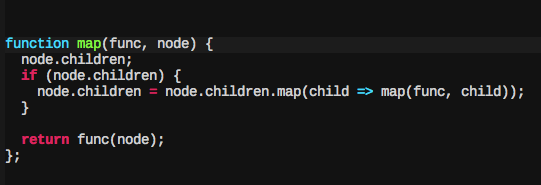
\includegraphics[height=1.7in]{figures/functor}
   \caption{Transcript Data Structure Map Function}
\end{figure}

The function passed to map must return a valid transcript tree node. Since each
function returns a the same type (tree node), we can compose multiple functions
for processing. This is important for separation of concerns and efficiency.
Functional composition allows us to write separate functions for tallying filler
words, calculating words per minute, formatting data, etc. Since the functions
are composed (see below) we only traverse the transcript tree once during our
processing.

% processTranscript = compose(
%   formatPopup,
%   countFilerWords,
%   wordsPerMinute,
% );
% 
% map(processTranscript, transcript);

% This code is equivalent to:

% wordsPerMinute(countFilerWords(formatPopup(transcript)))
\begin{figure}[H]
  \centering
   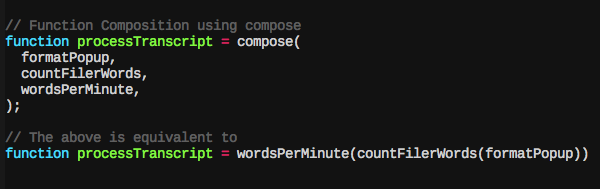
\includegraphics[height=1.7in]{figures/compose}
   \caption{Transcript Data Structure Compose}
\end{figure}

We use this pattern throughout the code base for processing transcript tree nodes.

\subsection*{Microservices}
\addcontentsline{toc}{subsection}{Microservices}

To address separation of concerns, allow for multiple languages, and lend the
system to easy scaling we chose a microservice based architecture. Our backend
consists of four microservices. 
 
 
\begin{figure}[H]
  \centering
   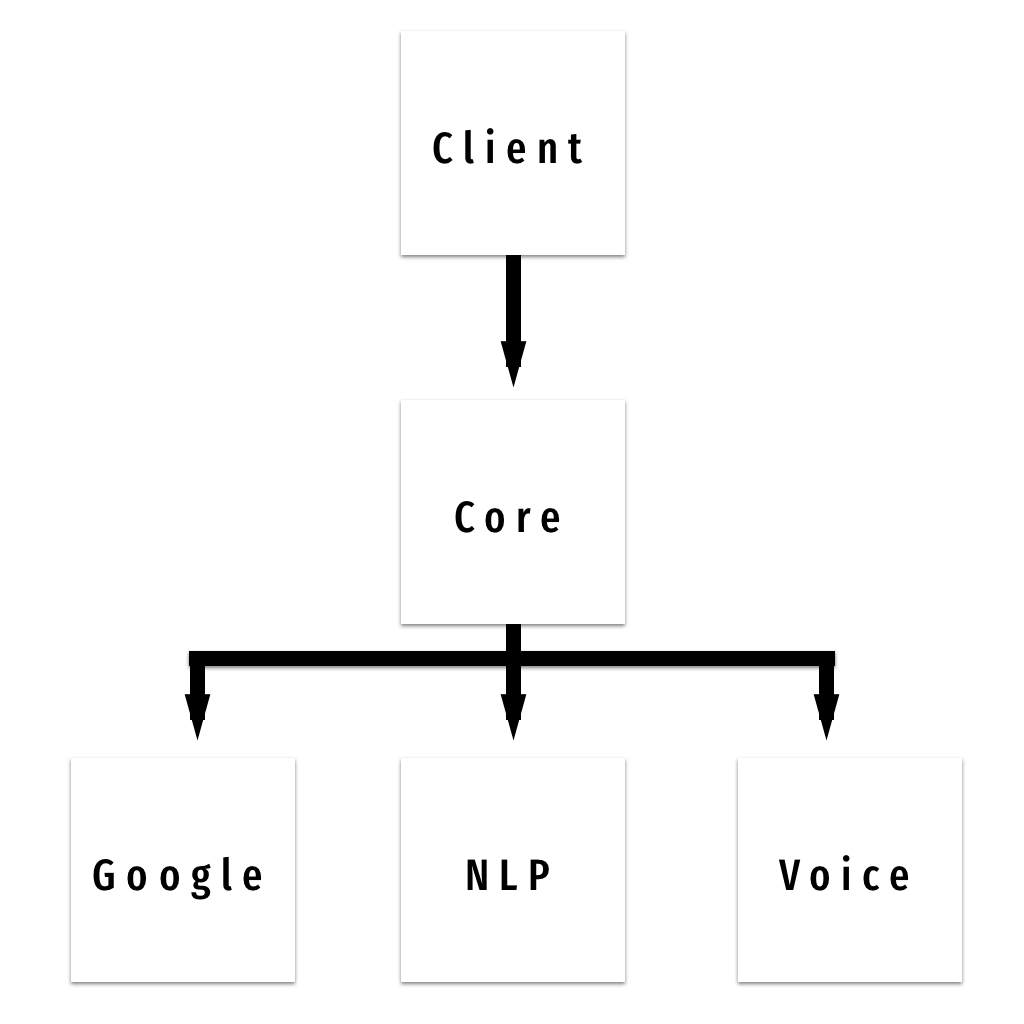
\includegraphics[height=3.7in]{figures/microservices}
   \caption{Microservice Architecture High Level Overview}
\end{figure}

Most of the application logic lies in the node.js service entitled core in the
figure above. The arrows represent the direction of requests and data in the
application. The core service is the main interface between the client and the
backend. We are using a session cookie based authentication scheme.
Authenticated requests pass through the core service. We use  asynchronous
processing upon video uploads to allow for near real time feedback to begin
populating the view. This necessitated a module that is capable of coordinating
requests and combining results. Jason Feng implemented the three backend
microservices that provide additional data processing API’s in python using
flask. A high level overview of the function of each service is as follows:


\begin{figure}[H]
  \centering
   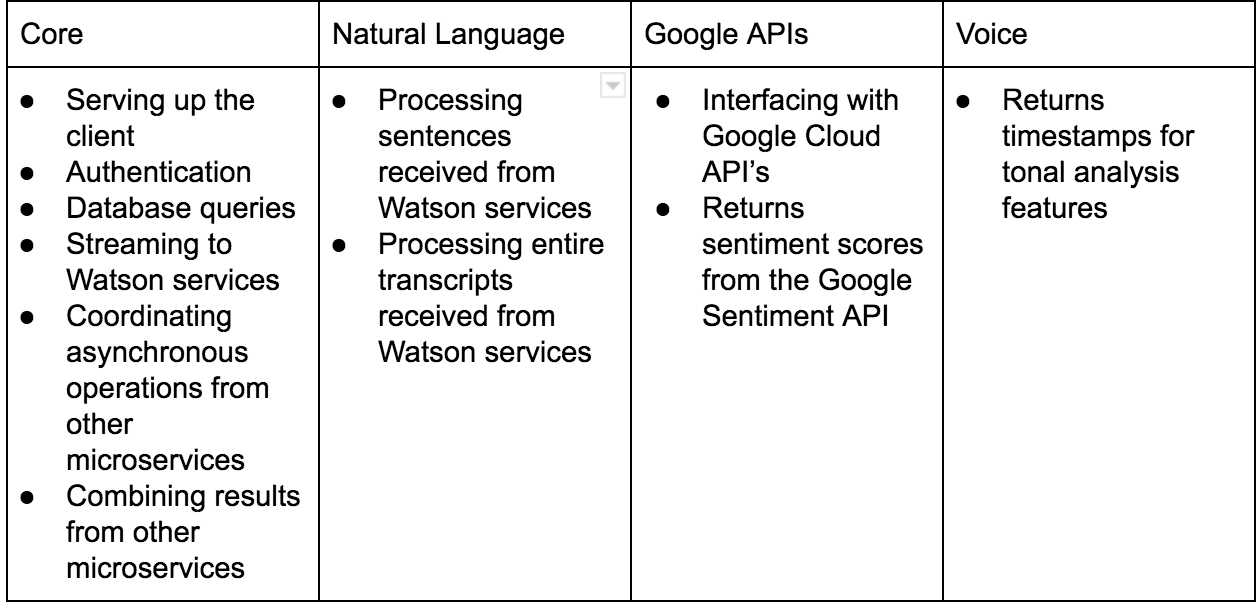
\includegraphics[height=3.0in]{figures/microservice_separation}
   \caption{Microservice Responsibilities High Level Overview}
\end{figure}

\subsection*{Client}
\addcontentsline{toc}{subsection}{Client}

\subsubsection*{Single Page Application}
\addcontentsline{toc}{subsubsection}{Single Page Application}

The client is a single page application built using React, a javascript
rendering framework. React uses functional components to split rendering logic.
We have coupled React with the popular state management framework Redux as well
as React Router for frontend routing. The routes we have implemented correspond
to the views discussed in the Design chapter.

\subsubsection*{Module Bundling and Loading}
\addcontentsline{toc}{subsubsection}{Module Bundling and Loading}

It was critical for our app to be fast and maintainable so we chose webpack as
our industry standard bundler. Webpack supports code splitting, a technique used
to deliver javascript to the browser as needed in single page applications. This
decreases the initial load time for each page by delivering smaller payloads,
thus combating page weight problems experienced by large applications.

\subsubsection*{Transcript Rendering}
\addcontentsline{toc}{subsubsection}{Transcript Rendering}

A crucial user interface element is the transcript. In order to display the
hierarchical structure discussed in the Data Structures section we use a depth
first traversal to render elements. This is necessary because we display
features as popups when the user hovers over a word or sentence. Sentence
features must be displayed when the user hovers over any portion of the tagged
sentence. Similarly, filler words should trigger a popup independent of the
surrounding sentence. The depth first traversal places each word in a span tag.
Each sentence is also a span tag with nested words.

\subsection*{Server}
\addcontentsline{toc}{subsection}{Server}

Node.js is a JavaScript environment that allows us to run JavaScript outside of
the browser. JavaScript is an asynchronous, non-blocking, event driven,
language. This model allows JavaScript to manage multiple requests/users in a
performant manner and hence makes it an invaluable language for client and
server-side web development.

The core microservice is built with node.js and express.js. Express is a popular
routing framework for node.js web applications that allows requests to be
serviced by middleware functions. It is critical that we use a framework that
lends itself to maintainability and scalability. The middleware reduces the need
for repeating logic and thus allows for DRY code on the server. Middleware
functions are registered to REST endpoints. The functions can be used to respond
to the request, pass it along, or handle error cases.

\textbf{MongoDB} is our NoSQL datastore of choice for storing documents.
 
\textbf{FFmpeg} is a cross-platform solution for video and audio recording and
conversion. FFmpeg can output the converted file on a stream which was
invaluable for our data processing pipeline performance.

\subsection*{Cloud Services}
\addcontentsline{toc}{subsection}{Cloud Services}

Pitchback’s backend is dependant upon multiple cloud services.
 
\textbf{Amazon S3} is our file storage platform. Video and presentation slide
uploads are stored and served from S3.
 
\textbf{Amazon Elastic Transcoder} converts user uploaded videos into an mp4
format that is accessible by all browsers. Files are converted from Amazon S3
and thumbnails are generated in periodic intervals.
 
\textbf{Watson Speech To Text} transcribes audio streams and returns
intermediate results with metadata such as timestamps and possible alternative
transcripts.

\subsection*{Data Flow}
\addcontentsline{toc}{subsection}{Data Flow}

\begin{figure}[H]
  \centering
   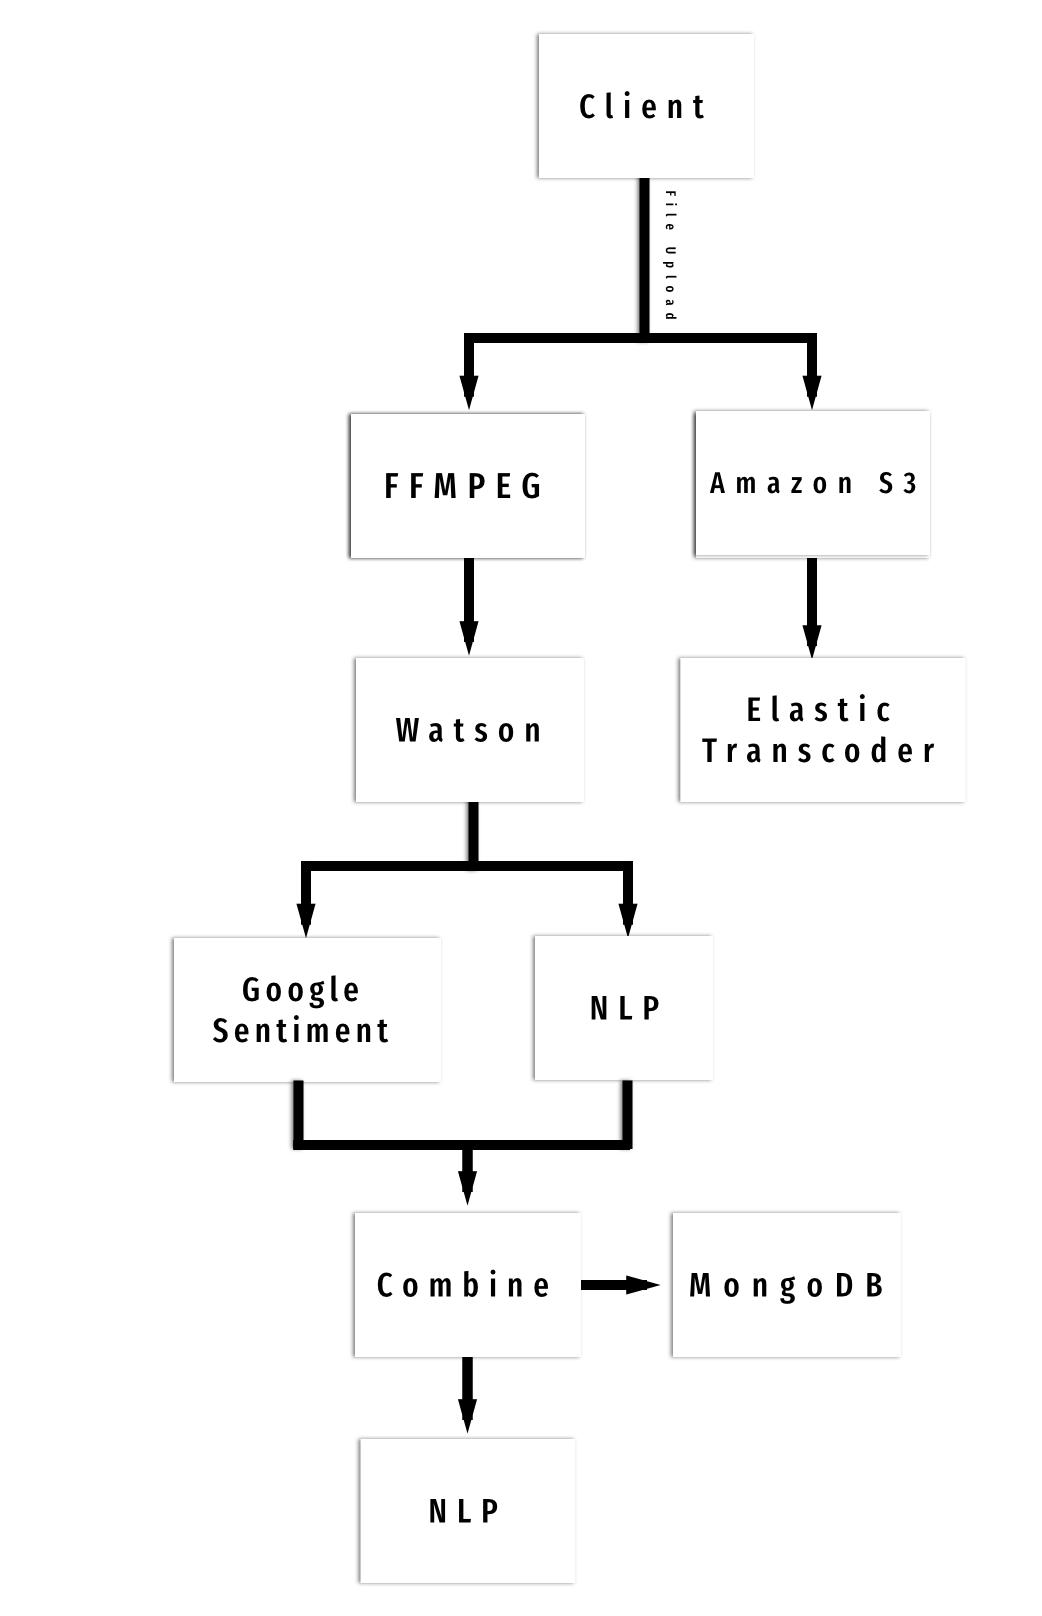
\includegraphics[height=7.5in]{figures/data_flow}
   \caption{Data Processing Pipeline}
\end{figure}

As previously mentioned, usability of the platform from a user perspective
entails performant data processing. To achieve the fastest possible results we
have designed a data flow model that runs computations asynchronously on two
independent streams: the file upload stream and the transcription analysis
stream. Both streams are initiated by a video upload. Upon video upload a
revision object is created in the database. While both streams store
intermediate results in the revision object. The frontend receives these
intermediate results by polling an endpoint on the core node.js service to
receive the most recent copy of the revision object.


\subsubsection*{File Upload Stream}
\addcontentsline{toc}{subsubsection}{File Upload Stream}

The video file stream is split and a piped to Amazon S3 via their multipart file
upload api. Upon completion the video is converted by the Amazon Elastic
Transcoder service. The transcoded video resource URL is stored under the
videoURL field in the revision database object.

\subsubsection*{Transcription and Analysis Stream}
\addcontentsline{toc}{subsubsection}{Transcription and Analysis Stream}

\paragraph{Conversion}
The video file stream is also piped to a child process running FFmpeg. This
child process converts the video stream into the wav audio format.

\paragraph{Transcription}
The Watson Speech to Text service exposes a websocket for transporting data and
receiving results. When the stream is created we initialize the transcript of
the current revision object. The output from the FFmpeg conversion is piped to
Watson. In Node.js streams are event emitters. The Watson stream exposes two
events of interest: results and close. The results event fires with intermediate
results from Watson. These results are the transcript of a sentence unit. A
sentence unit is a portion of the audio for which there is no sufficient pause
in speech. We heuristically create sentence nodes with their child word nodes
from these sentence units.

\paragraph{Sentence Tagging}
Each results event from the Watson stream triggers two concurrent post requests
for sentence feature tagging. The first is a request to the natural language
processing microservice at its \textbf{/grammar/sentence} route. The child word nodes of
the sentence node may contain filler, weak-word, adverb, or, adjective. The
second request is to the google sentiment microservice at its
\textbf{/language/sentiment} route. The sentence node may contain the tag sentiment with
a value ranging from -1 to 1. This value is the score given by the google
service on a scale of negative to positive sentiment.

\paragraph{Combine}
To coordinate these requests we are using the Promise API, a popular JavaScript
pattern for managing asynchronous code. The promise API wraps asynchronous code
and provides two functions: then and catch. The user provides a function when
the promise is created to deal with success and failure cases respectively
called resolve and reject. The then function is called on success with an
optional single argument determined by the user. The error function is similarly
called on failure. Promises are in one of three states at any given time:
pending, resolved, or rejected.  Both sentence tagging requests are wrapped in
Promises. We use the Promise.all function which takes a list of promises as an
argument. Promise.all waits for each promise to resolve before calling then.
Therefore we pass our two sentence tagging requests to Promise.all as a list and
wait for both responses.

Upon receiving both responses we now have two separate transcripts both
representing the same revision but with different features tagged on its
sentence and word nodes. Therefore we need to combine both transcripts into one
before persisting to the revision database object. To combine the transcripts we
take advantage of the unique keys on each node of the tree. Arbitrarily we
traverse the sentiment sentence tree first and create an inverted index of key
to node for a sentence if the absolute value of the sentiment score is greater
than 0.4. The filter's purpose is to tag sentences that have either a strong
positive or negative sentiment and ignore those that are more or less neutral.
After we have created this index we traverse the sentence tree returned from
natural language processing. For each node, if the current key is in the
inverted index combine the feature dictionaries of both nodes. Note that we
traverse two shallow trees of depth 2 to  generalize the algorithm. The
generalized algorithm allows for a more complex data flow in the future with the
possibility of sending entire paragraphs for more context in sentiment and
grammar analysis. It is easy to see that both trees are traversed once and
therefore the combination algorithm runs in O(n) time. While traversing the
natural language processing sentence node we maintain counters for each feature
and its corresponding word. This count will make insertion into the overall
transcript more efficient as we will soon see.

The combined sentence tree must be persisted to the revision database object for
intermediate results to begin rendering on the frontend. There are two cases: we
currently have the first sentence or there is an existing transcript in the
database from previous cycles of this process. The first case is trivial in that
we simply create a transcript node, insert the current sentence as the first
child node of the transcript, and use all of its metadata as the metadata for
the entire transcript. In the second case, we are adding a sentence node to a
transcript tree. Thus, we must shift the indices of all nodes to be relative to
the transcript rather than to the sentence itself. We must also add the feature
count of the sentence to the total feature count of the transcript. Finally, the
end timestamp of the transcript must be revised to the end of the final word of
the current sentence. Since we update each child node of the current sentence to
shift the metadata relative to the transcript, this step also runs in O(n) time.

\paragraph{Transcript Tagging}
The Watson close event signals the end of the file stream and the completion of
transcription. Similar to the logic for combining the API calls, we use
Promise.all to wait for the final requests and combine steps to be completed.
Once complete we make a request with the entire transcript to the
/grammar/groups route of the natural language service for higher level feature
tagging for which the entire transcript may be necessary. This service returns a
transcript with sentence nodes possibly tagged as passive and/or weak-phrase.
Using our tagged transcript, we do a final pass over the tree to calculate the
words per minute for the presentation.

The final transcript is persisted to the database and the revision processing
field is marked as finished to signal the frontend to stop polling.

\section*{Discussion and Results}
\label{chapterdiscussionandresults}
\addcontentsline{toc}{section}{Discussion and Results}

\subsection*{Data Processing Performance}
\addcontentsline{toc}{section}{Data Processing Performance}
As previously discussed, the processing of our feedback in a performant manner
was of the utmost importance in order to create a usable platform. In
implementing our multiple stream data processing pipeline we saw significant
performance improvements over prior attempts to analyze videos serially. A major
contribution to this performance increase was the ability to display
intermediate results on the client. This feature made our application feel much
faster.

\subsection*{User Feedback}
\addcontentsline{toc}{section}{User Feedback}
In informal discussions with 12 users of the platform we have found that users
find our presentation insights useful. Choosing material design created a look
and feel that users are already familiar with due to its popularity. Therefore,
users were generally able to navigate our platform without an onboaring tutorial
user flow. Our insights are presented inline with the transcript. Users found
this presentation of the data to be helpful in navigating and consuming our
feedback. An obvious extension to this work would be to launch a larger beta
test.

\section*{CONCLUSION AND FUTURE WORK}
\label{chapterfuturework}
\addcontentsline{toc}{section}{Future Work}

\subsection*{Transcript}
\addcontentsline{toc}{subsection}{Transcript}
The effectiveness of our platform is clearly limited by the quality of the video
transcript. To mitigate this issue we propose three extensions: incorporating
watson alternative results, allowing users to edit and reprocess the transcript,
and a paragraph transcript tree node.

\subsubsection*{Watson Alternative Results}
\addcontentsline{toc}{subsubsection}{Watson Alternative Results}

The \textbf{Watson Speech to Text} service returns a list of words during the
transcribing process in order of confidence. We simply use the highest
confidence word to assemble a sentence. It is rare that the correct transcript
for a given presentation is comprised of solely top confidence words. An obvious
extension would be to consider all of the possible words to create our
transcript. A system for doing so could include exposing these options to the
user in a drop down menu, or using grammar and context to select a word from the
list.

\subsubsection*{Edit Transcript and Reprocess}
\addcontentsline{toc}{subsubsection}{Edit Transcript and Reprocess}
Integrating a feature into the current user interface for editing and
reprocessing the transcript is another option for increasing the quality of the
transcript. If users may edit their transcripts, the transcript tree data
structure must implement insert, update, and delete.

\subsubsection*{Paragraph Tree Node}
\addcontentsline{toc}{subsubsection}{Paragraph Tree Node}
Creating another transcript tree node type paragraph, may be beneficial for data
processing. Paragraph nodes would allow for specific contextualization of the
sentence child nodes for feature detection. Creating this node would require
advanced natural language processing techniques to identify topic changes in a
presentation transcript.

\subsection*{Voice Insights}
\addcontentsline{toc}{subsection}{Voice Insights}
Effective communication and engaging presentation style encompasses more than
word choice. Jason Feng has implemented a microservice that generates timestamps
for tonal features such as monotone and rising tone. An obvious next step would
be to integrate this service into the data processing pipeline. A challenge in
doing so is matching timestamps with word and sentence nodes in the transcript
tree in a performant manner. Tonal processing is independent of the file upload
and transcription analysis streams. Tonal processing would therefore run on its
own stream adding to the asynchronous processing complexity.

\subsection*{Trends}
\addcontentsline{toc}{subsection}{Trends}
Insights are limited to the scope of an individual take of a presentation.
Pattern recognition across takes requires a new tree structure that is a
collection of transcript trees. This new tree facilitates processing feature
trends over time and a greater context for understanding the presentation.

\subsection*{Group Permissions}
\addcontentsline{toc}{subsection}{Group Permissions}
Our sharing feature publishes a take to the entire user base. It would be
convenient for groups of users to publish takes to each other. This feature
would facilitate Pitchback’s use with classes, student groups, companies, teams,
etc.

% 
% You can discuss each study separately under this section. 
% 
% \subsection*{User Study 1: Where We Prove Everything}
% \addcontentsline{toc}{subsection}{User Study 1: Where We Prove Everything}
% 
% This user study was dope.
% 
% It follows that there are four cases that can occur.  This is just a random paragraph as paragraphs go. There is something here that will sound sciency.
% 
% \begin{itemize}
% \item \textbf{True Positive:} it really happened
% \item \textbf{False Positive (Type I error):} it didn't happen but they thought it did
% \item \textbf{True Negative:} didn't happened
% \item \textbf{False Negative (Type II error):} happened but they deny it
% \end{itemize}
% 
% Throw in some Bayes' theorem. We know that $P(A \mid B) = \frac{P(B\mid A)P(A)}{P(B)}$. Then use some tables. As much of your results should be shown in table form. 
% 
% \begin{table}[h!]
%   \begin{center}
%     \begin{tabular}{|c||c|c|c|}
%     \hline
%     Total Fixation Duration on Element(s) & Report Yes & Report No & Total\\ \hline \hline
%     $>0.0-0.5$ & 523 & 542 & 1070 \\ \hline 
%     $>0.5-1.0$ & 452 & 265 & 723 \\ \hline
%     $>1.0-1.5$ & 214 & 127 & 341 \\ \hline
%     $>1.5-2.0$ & 125 & 62 & 187 \\ \hline
%     $>2.0-2.5$ & 72 & 27 & 99 \\ \hline
%     $>2.5-3.0$ & 48 & 12 & 60 \\ \hline
%     $>3.0$ & 75 & 16 & 91 \\ \hline
%     Total & 1509 & 1051 & 2571 \\ \hline
%     \end{tabular}
%   \end{center}
%   \caption{Table of data}
% \end{table}
% 
% Throw in some more graphs.
% 
% \begin{figure}[h!]
%   \centering
%   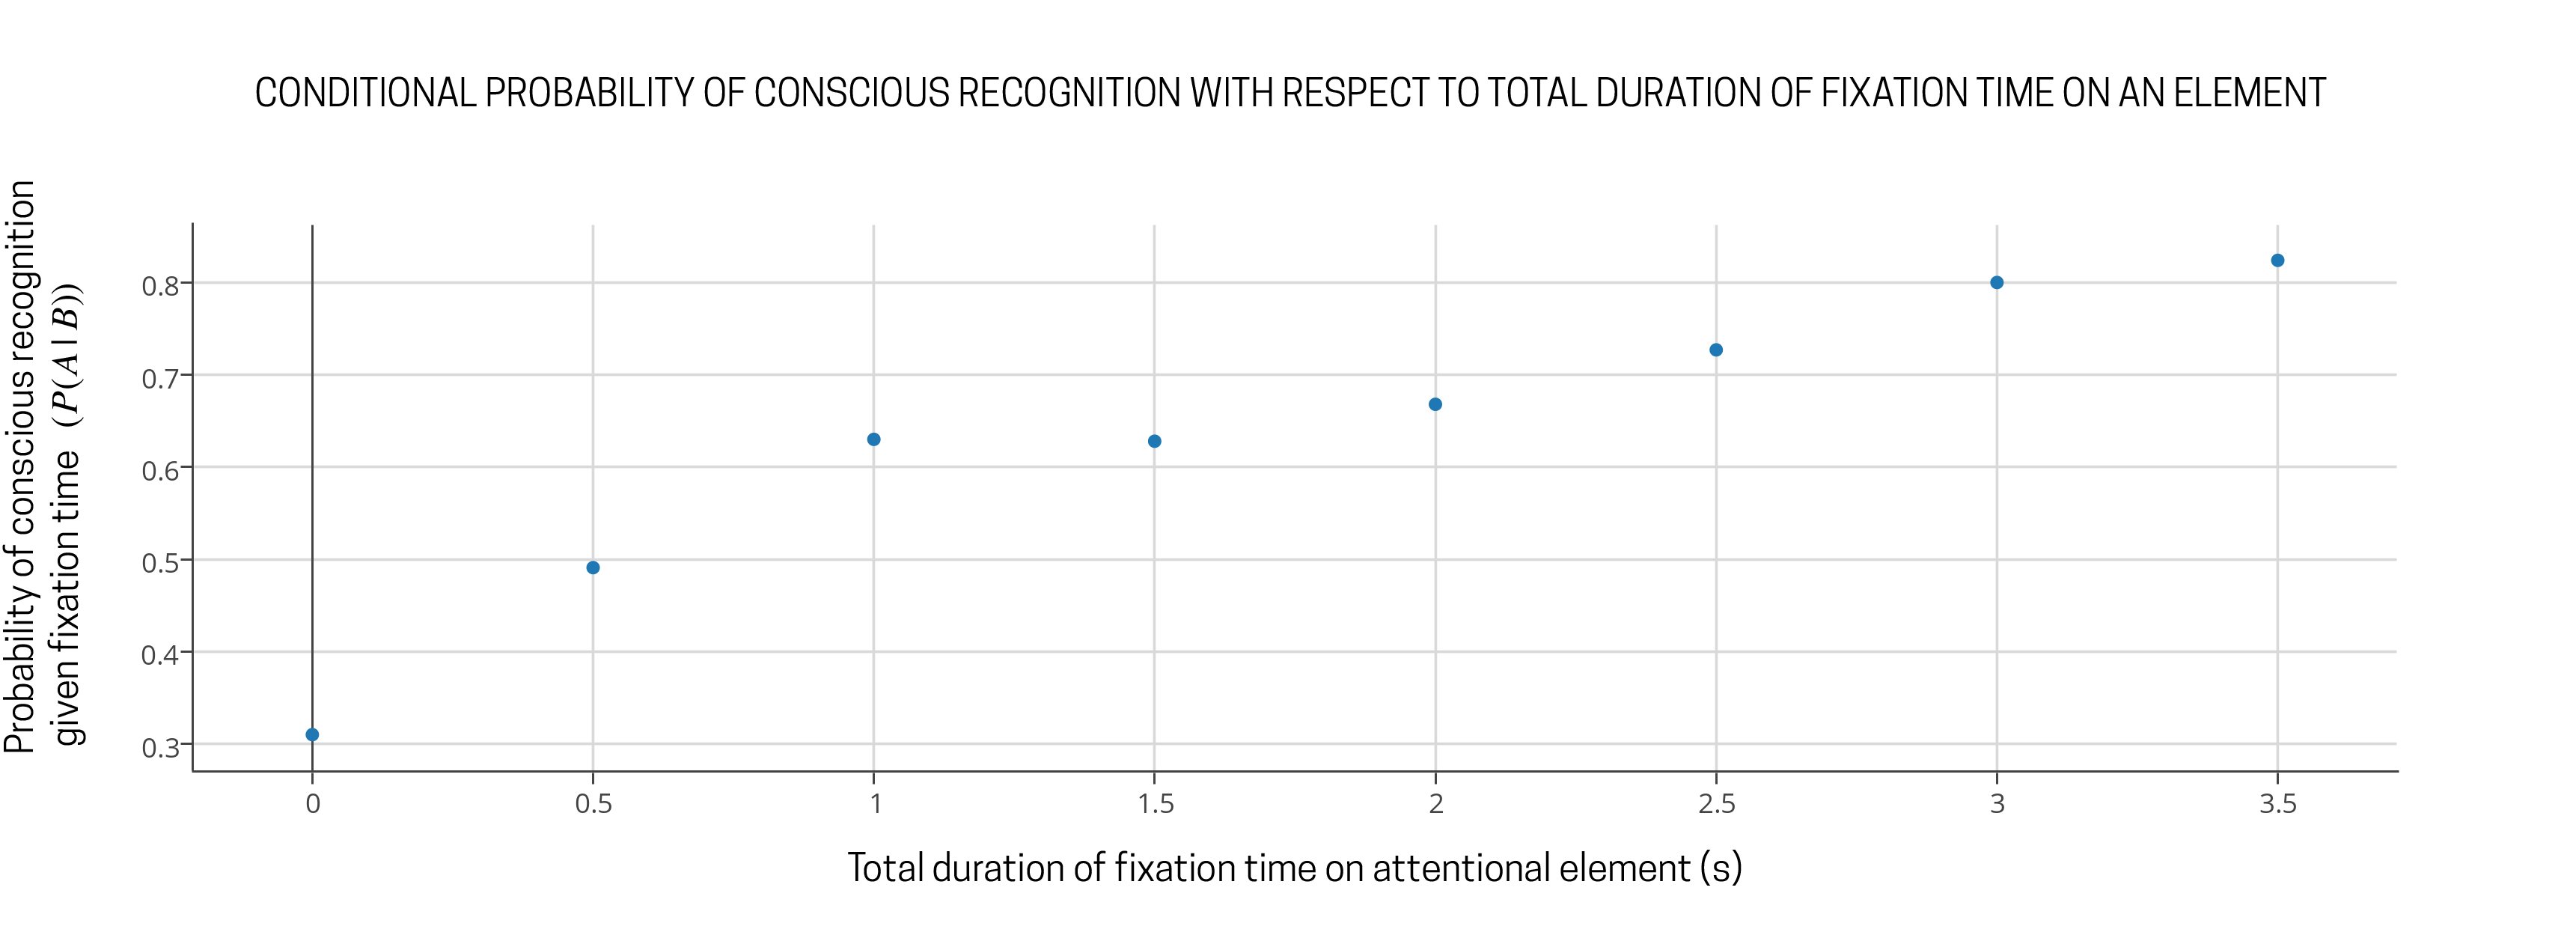
\includegraphics[height=2 in]{figures/recallprob.png}
%   \caption{Graphs are fun}
% \end{figure}
% 
% 
% \begin{table}[h!]
%   \begin{center}
%     \begin{tabular}{| c || c | c |}
%     \hline
%     Group & A & B \\ \hline \hline
%     Mean & 0.329182223909 & 0.747958949667 \\ \hline
%     Standard Deviation (SD) & 0.310879429427 & 0.047694993705  \\ \hline
%     Standard Error of the Mean (SEM) & 0.093733674768 & 0.027536717454  \\ \hline
%     Population Size (N) & 110 & 30  \\
%     \hline
%     \end{tabular}
%   \end{center}
%   \caption{Analysis of things}
% \end{table}
% 
% 
% Our results show that we are right — the answer is beyond a doubt 42. You are welcome.

%\include{Chapter2}          % continue to include all the chapters.

% \appendix
% 


\section*{Appendix A: User Study 1}
\addcontentsline{toc}{section}{Appendix A: User Study 1}


Study Results:

\begin{table}[h!]
\centering
 \begin{tabular}{|m{5em} || m{6em} | m{10em} | m{10em}|} 
 \hline
 col1 & col2 & col3 & col4 \\ 
 \hline\hline
 stuff & 0.0516810976 & stuff & more stuff \\ 
 [1ex] 
 \hline
 \end{tabular}
\end{table}






\singlespacing

\bibliography{myrefs}
\addcontentsline{toc}{section}{Bibliography}

\end{document}
